\documentclass[conference,10pt]{IEEEtran}

% For arXiv submission: declare CC BY 4.0 license via the arXiv submission form's
% license selector (recommended) or by adding a footnote after \maketitle.
% LICENSE: This work is licensed under CC BY 4.0 (https://creativecommons.org/licenses/by/4.0/).
\IEEEoverridecommandlockouts

\usepackage[T1]{fontenc}
\usepackage[utf8]{inputenc}
\usepackage{cite}
\usepackage{amsmath,amssymb,amsfonts}
\usepackage{algorithmic}
\usepackage{graphicx}
\usepackage{textcomp}
\usepackage{xcolor}
\usepackage{url}
\usepackage{booktabs}
\usepackage{array}
\usepackage{multirow}
\usepackage{tikz}
\usetikzlibrary{arrows.meta,positioning,shapes.geometric,fit,calc,shapes.misc}
\usepackage{hyperref}

\newtheorem{proposition}{Proposition}
\newtheorem{remark}{Remark}

\def\BibTeX{{\rm B\kern-.05em{\sc i\kern-.025em b}\kern-.08em
    T\kern-.1667em\lower.7ex\hbox{E}\kern-.125emX}}

\hypersetup{%
  pdftitle={Byzantine-Fault-Tolerant Hierarchical Navigation for GNSS-Denied UAV Swarms: Architecture, Theoretical Analysis, and Evaluation Methodology},%
  pdfauthor={Oleksandr Kalynovskyi},%
  pdfsubject={UAV swarm cooperative localisation, Byzantine fault tolerance, Terrain-Referenced Navigation},%
  pdfkeywords={BFT, UAV swarm, cooperative localisation, iSAM2, GTSAM, TRN, Sybil detection}%
}

\begin{document}
\pagestyle{plain}

\title{Byzantine-Fault-Tolerant Hierarchical Navigation\\ for GNSS-Denied UAV Swarms:\\ Architecture, Theoretical Analysis, and Evaluation Methodology\thanks{The methods described in Sections~\ref{sec:approach}-B through~\ref{sec:approach}-G are the subject of pending patent applications filed with the German Patent and Trademark Office (DPMA), Aktenzeichen 10~2026~001~712.2 and a related application. This manuscript describes the technical content of those filings for the purposes of academic disclosure. \emph{Note}: this paper presents the architecture, formal analysis, and a complete simulation methodology; empirical validation is deferred to future work where the proposed methodology will be executed in a Gazebo/ROS2-based simulation framework currently under development.}}

\author{\IEEEauthorblockN{Oleksandr Kalynovskyi}
\IEEEauthorblockA{Independent Researcher\\
Email: kalinovsky.research@proton.me}}

\maketitle

\section*{Abstract}
Cooperative navigation of unmanned aerial vehicle (UAV) swarms under Global Navigation Satellite System (GNSS) denial has advanced rapidly, but most deployed systems implicitly assume that every peer reports honestly; adversarial-peer defence at the state-estimation layer is largely absent. We present an architecture that, to our knowledge, is the first to simultaneously address six concerns previously treated in isolation: (1)~Byzantine-fault-tolerant (BFT) consensus over navigation data, (2)~a hierarchical anchor/follower topology with dynamically assigned roles, (3)~reputation-weighted multi-hop position relay, (4)~automatic failover with sub-10-second design budget, (5)~GNSS-spoofing detection through ultra-wideband (UWB) cross-verification, and (6)~load balancing under progressive attrition. Based on a systematic review of approximately 90 publications (2020--2026), no prior work combines all six within a flight-grade continuous-state estimator---where \emph{flight-grade} denotes sub-50\,ms optimisation latency, sub-15\,kbit/s per-UAV bandwidth, and sub-100\,m circular error probable (CEP) at cruise speeds $\geq$30~m/s. The core primitive is a \emph{Visual Proof of Observation}: cryptographically signed hashes of terrain feature descriptors that neighbouring UAVs verify by physical revisit. Reputation is updated asymmetrically ($\alpha_\text{neg}\!\geq\!2\alpha_\text{pos}$) and mapped to factor-graph noise covariances. We derive a Byzantine safety bound and a convergence bound for na\"ive-Byzantine exclusion (the formal safety guarantees apply to na\"ive adversaries; partial mitigation against strategic adversaries is discussed but not formally proved) and quantify per-hop error propagation in closed form; under the recommended parameter set, the analysis predicts exclusion of a compromised anchor on the order of a few hundred seconds, sub-10-s follower reassignment after anchor loss, and CEP $<$100~m up to three relay hops under multi-anchor fusion (the default operating mode). To support reproducible evaluation, we present a complete simulation methodology (six experiments covering CEP-vs-hops, failover timing, Byzantine exclusion, GNSS-spoofing reaction, progressive attrition, and ablation) together with the analytical predictions each is designed to validate. Empirical execution of the methodology in a Gazebo/ROS2 framework, hardware-in-the-loop validation, and head-to-head comparison against the original SwarmRaft implementation are deferred to future work.

\begin{IEEEkeywords}
UAV swarm, Byzantine fault tolerance, GNSS-denied navigation, factor graph, reputation
\end{IEEEkeywords}

\section{Introduction}
\label{sec:intro}

\IEEEPARstart{U}{nmanned} aerial vehicle (UAV) swarms are increasingly deployed in contested environments where GNSS signals are unavailable, degraded, or deliberately denied. Recent operational experience in military and civil domains has underscored two coupled vulnerabilities: GNSS-dependent navigation collapses under electronic warfare, and cooperative navigation schemes that share position information between vehicles assume that every participant reports honestly. A single compromised UAV---captured, sensor-faulted, or infected with malicious firmware---that transmits falsified odometry or absolute-position estimates can corrupt the navigation solution of the entire swarm without detection.

Three research streams have independently matured in the past five years. First, cooperative GNSS-denied navigation has produced flight-grade systems such as the Distributed PNT Chain~\cite{shapero2023distributed}, Omni-swarm~\cite{xu2022omniswarm}, Kimera-Multi~\cite{tian2022kimera}, and Swarm-SLAM~\cite{lajoie2024swarmslam}, and anchor-free multi-sensor fusion schemes such as DTVIRM-Swarm~\cite{dtvirm2026} have added magnetic and monocular cues. Second, Byzantine-fault-tolerant (BFT) protocols for robot swarms have evolved from abstract consensus~\cite{strobel2020blockchain} to deployed token economies~\cite{strobel2023robot} and blockchain-secured cluster hierarchies~\cite{alsamhi2023blockchain}. Third, reputation and trust frameworks for multi-agent systems have converged on asymmetric update rules and physical-layer observations~\cite{yemini2022characterizing,mallmanntrenn2022crowd,ballotta2025confidence}. Yet these streams have not merged at the flight-control layer. The two 2025 systems closest to a unified architecture---SwarmRaft~\cite{dev2025swarmraft} and the Byzantine Distributed GPS Detection (BDGD) algorithm~\cite{zhong2025bdgd}---each cover at most three of the design dimensions required for a deployable solution; an earlier and largely complementary system, the Byzantine Follow-The-Leader (BFTL) formalism of Castelló~Ferrer~\emph{et~al.}~\cite{castelloferrer2022bftl}, covers four, but operates on discretised maps rather than a continuous flight-grade state estimator.

This paper introduces a navigation architecture that simultaneously addresses six pillars: (i)~BFT consensus over shared state, (ii)~a hierarchical anchor/follower topology with roles assigned dynamically in flight, (iii)~reputation-weighted multi-hop position relay, (iv)~automatic failover within 10~seconds of anchor loss, (v)~GNSS-spoofing detection via UWB cross-verification, and (vi)~load balancing across anchors under progressive attrition. Based on a systematic review of approximately 90 publications spanning 2020--2026 across Byzantine-fault-tolerant swarms, GNSS-denied cooperative navigation, multi-robot reputation systems, hierarchical swarm control, GNSS-spoofing detection, and multi-hop position relay (see Section~\ref{sec:related} footnote for review methodology), we find, to our knowledge, no published system integrating more than four of these pillars, and none doing so within a continuous-state flight-grade factor-graph estimator. The architecture rests on a new primitive, the \emph{Visual Proof of Observation} (PoO): each terrain-relative navigation (TRN) fix produces a cryptographically signed record containing a hash of terrain feature descriptors, which neighbouring UAVs verify by comparing their own descriptors when they later fly over the claimed region. Because feature descriptors are physically bound to terrain, illumination, and the learned extractor network, they cannot be fabricated by a vehicle that has not actually observed the location, distinguishing this mechanism from signal-level or purely statistical trust.

Our contributions are as follows. \emph{First}, we formulate a visual PoO mechanism that gives distributed navigation a terrain-anchored verification primitive (physically bound to terrain, illumination, and the learned feature extractor; unforgeable in the practical sense under the threat model of Section~\ref{sec:model}, although not under the formal cryptographic UF-CMA definition), and we show how to integrate signed observations into an incremental smoothing and mapping (iSAM2) factor graph as reputation-weighted priors alongside UWB ranging factors. \emph{Second}, we define an asymmetric reputation rule ($\alpha_\text{neg}\!\geq\!2\alpha_\text{pos}$, preferably $3{:}1$) that excludes Byzantine participants faster than honest peers accumulate trust while tolerating transient verification failures from environmental degradation. \emph{Third}, we introduce a dynamic anchor-score assignment combining reputation, TRN confidence, imagery coverage, and load, together with a ``request--offer--select'' failover protocol with bounded recovery time. \emph{Fourth}, we derive a safety condition for quorum-based exclusion, expose its limits when the quorum parameter $M$ is fixed, give a closed-form expected-time bound for na\"ive-Byzantine exclusion, and present a closed-form per-hop error-growth model. \emph{Fifth}, we present a complete simulation evaluation methodology (six experiments covering CEP-vs-hops, failover timing, Byzantine detection and exclusion, GNSS-spoofing reaction, progressive attrition, and ablation), each paired with the analytical prediction it is designed to validate; empirical execution of this methodology is deferred to future work in a Gazebo/ROS2 framework currently under construction.

The remainder of the paper is organised as follows. Section~\ref{sec:related} surveys related work. Section~\ref{sec:model} formalises the system and threat model. Section~\ref{sec:approach} details the proposed approach in seven subsections. Section~\ref{sec:theory} presents the theoretical analysis. Section~\ref{sec:sim} presents the proposed evaluation methodology with the analytical prediction each experiment is designed to test. Sections~\ref{sec:asym-decay-empirical}, \ref{sec:clamp-convergence-empirical}, and \ref{sec:byzantine-scaling-empirical} report three abstract Monte Carlo validation studies of the asymmetric reputation rule, the convergence bound, and Byzantine-fraction resilience respectively. Section~\ref{sec:discussion} discusses limitations and deployment considerations. Section~\ref{sec:conclusion} concludes.

\section{Related Work}
\label{sec:related}

We organise prior art into five domains and summarise design-space coverage of the most relevant systems in Table~\ref{tab:coverage}.\footnote{Review methodology: candidate publications were identified by keyword search in Google Scholar, arXiv, IEEE Xplore, and ACM Digital Library between February and April 2026 using combinations of \{\emph{Byzantine, BFT, fault-tolerant, reputation, trust}\} $\times$ \{\emph{UAV, drone, swarm, multi-robot}\} $\times$ \{\emph{navigation, localisation, SLAM, GNSS, GPS}\}; inclusion criteria were peer-reviewed conference or journal venue (or arXiv preprint with an identifiable author affiliation), publication date 2020--2026, and at least partial coverage of one of the six pillars enumerated in Section~\ref{sec:intro}. Of approximately 90 candidate publications screened, the systems explicitly compared in Table~\ref{tab:coverage} are those that cover three or more pillars. The ``to our knowledge'' hedge in the abstract and conclusion reflects the irreducible incompleteness of any keyword-based search.}

\subsection{Byzantine Fault Tolerance in UAV Swarms}

The Byzantine fault model originates with Lamport, Shostak, and Pease~\cite{lamport1982byzantine}, who established the foundational $n \geq 3f+1$ requirement for consensus among $n$ peers in the presence of $f$ arbitrarily-faulty participants. Practical implementations have evolved through two main families described below.

\textbf{Raft-family adaptations.} The original Raft consensus algorithm~\cite{ongaro2014raft} provides crash-fault tolerance with leader-based replication; UAV-specific extensions add Byzantine resilience on top of this substrate. SwarmRaft~\cite{dev2025swarmraft} performs median-based correction of spoofed GNSS positions among leader-collected peer reports and includes a Byzantine-resilient evaluation step on top of a crash-fault Raft core. Its design choice is not presented as a limitation by the authors, but the system lacks persistent reputation across rounds, weights all peers equally within a round, and retains a single elected leader. Zhang~\emph{et~al.}~\cite{zhang2024reputation} overlay Proof-of-Authority on Raft for UAV routing, not localisation. Zuo~\emph{et~al.}~\cite{zuo2022voting} provide Raft-inspired leader election with explicit follower-loss failover but no reputation.

\textbf{PBFT variants.} Practical Byzantine Fault Tolerance, originally introduced by Castro and Liskov~\cite{castro1999pbft}, has spawned a family of UAV-specific extensions. LAP-BFT~\cite{kong2022lapbft} provides lightweight asynchronous BFT with vector commitments over 50 UAVs; DTPBFT~\cite{han2024dtpbft} extends PBFT with a dynamic trust mechanism for UAV swarms; ACBFT~\cite{wang2025acbft} is an adaptive chained Byzantine-fault-tolerant consensus protocol for UAV ad-hoc networks; DPoS-PBFT~\cite{hafeez2024dposbft} hybridises delegated proof-of-stake with PBFT finality. The concurrent reputation-enhanced PBFT variant RePA~\cite{repa2025iot} adds trust scoring to defend against node-capture attacks at the network layer. Concurrent work on parallelised BFT for swarm robots (PTEE-BFT~\cite{wang2025pteebft}) introduces a parallel-execution Byzantine consensus protocol for blockchain-secured swarms, addressing throughput rather than navigation. None of these targets localisation. The recent COUAVChain~\cite{couavchain2025}, an RB-HotStuff-based variant building on the HotStuff BFT protocol~\cite{yin2019hotstuff}, couples dynamic reputation, Bayesian inference, and hierarchical sharding for denied environments---architecturally closest to ours on the consensus side---but does not close the loop with spoofing detection or multi-hop position relay.

\textbf{Blockchain-based swarm reputation.} The IRIDIA/ULB line established Byzantine resilience for physical robot swarms~\cite{strobel2020blockchain,strobel2023robot,vancalck2023cooperation,dorigo2024nature}. Strobel~\emph{et~al.}~\cite{strobel2023robot} demonstrated a token economy on Pi-puck swarms that excludes adversaries autonomously. Castelló~Ferrer~\emph{et~al.}~\cite{castelloferrer2021secure} extended the framework with secure multi-party computation for confidential missions. Among these, the BFTL system~\cite{castelloferrer2022bftl} is the closest prior navigation-aware work: it formalises the Byzantine Follow-The-Leader problem, publishes cryptographically weighted routes to a blockchain, and proves completion bounds under Byzantine leaders and followers (including a form of leader-failure tolerance arising from the completion guarantees). BFTL covers BFT, hierarchy, reputation, and position relay but operates over discretised graph-structured environments (with routes committed to blockchain) rather than a continuous probabilistic factor-graph state estimator. The blockchain settlement layer used in the published BFTL demonstration has route-commitment finality on the order of seconds per round~\cite{strobel2020blockchain} --- a property of the chosen settlement layer rather than of the BFTL formalism itself, but the published instantiation as deployed is consequently incompatible with 50-ms control cycles; a future BFTL implementation over a faster settlement layer could in principle close this gap, and the BFT design choices that distinguish our work from BFTL are independent of the settlement-layer latency question (continuous-state factor-graph estimation, dynamic failover, and load balancing in particular). Alsamhi~\emph{et~al.}~\cite{alsamhi2023blockchain} link blockchain trust to cluster-head hierarchy with energy awareness but without multi-hop relay or spoofing defence. Jensen~\emph{et~al.}~\cite{jensen2019blockchain} and De~Campos~\emph{et~al.}~\cite{decampos2021iota} explored earlier blockchain-UAV integrations.

\textbf{Distributed resilient estimation.} The W-MSR track originating with LeBlanc~\emph{et~al.}~\cite{leblanc2013resilient}, with later extensions to trusted-node settings by Mitra~\emph{et~al.}~\cite{mitra2019resilient}, provides formal scalar-state guarantees but lacks flight-grade sensor-fusion detail.

\subsection{GNSS-Denied Cooperative Navigation}

The Distributed PNT Chain~\cite{shapero2023distributed} from GTRI factors a centralised Kalman filter over swarm poses into an undirected acyclic Bayes graph, matching centralised accuracy at $\sim$22\% of the compute cost. It does not defend against peers that falsify odometry---a spoofed node propagates unchecked through the factor graph. Omni-swarm~\cite{xu2022omniswarm} and its successor D\textsuperscript{2}SLAM~\cite{xu2022d2slam} are canonical decentralised UWB+VIO systems; CCM-SLAM~\cite{schmuck2019ccmslam}, COVINS~\cite{schmuck2023covinsg}, Kimera-Multi~\cite{tian2022kimera}, and Swarm-SLAM~\cite{lajoie2024swarmslam} are the leading collaborative VIO/SLAM frameworks, evaluated on swarms of fewer than 20 agents. None defends against falsified loop closures or odometry; statistical outlier rejection (GNC, robust kernels) is routine, but deliberate adversarial behaviour is out of scope. Moroncelli~\emph{et~al.}~\cite{moroncelli2024byzantine} extended Swarm-SLAM with blockchain-based geometric Byzantine detection---the closest prior coupling of reputation with SLAM, although operating on ground robots and without hierarchical failover.

The ``Collaborative Integrated Navigation'' scheme of Zhang~\emph{et~al.}~\cite{zhang2025collaborative} models uncertainty propagation from a leader to followers via UWB ranging but employs only two hierarchy levels with a statically assigned leader, no reputation, and no failover. The air--ground scheme of Yue~\emph{et~al.}~\cite{yue2025airground} uses high-altitude UAVs as fixed-role mobile UWB anchors without dynamic election, reputation propagation, or failover. DTVIRM-Swarm~\cite{dtvirm2026} is the most comprehensive honest-peer anchor-free fusion to date (MIMU + magnetic + monocular + UWB with $\chi^2$ outlier filtering), but assumes statistical rather than adversarial outliers.

\subsection{Reputation Systems for Multi-Robot Systems}

Yemini~\emph{et~al.}~\cite{yemini2022characterizing} injected stochastic physical-layer trust into consensus, breaking the classical $<\!50\%$ malicious bound. Ballotta~\emph{et~al.}~\cite{ballotta2025confidence} added time-decaying confidence for tunable convergence. Mallmann-Trenn, Cavorsi, and Gil~\cite{mallmanntrenn2022crowd} extended this idea to flocking through ``crowd vetting'' of trust opinions. FLTrust~\cite{cao2021fltrust} is the federated-learning analogue. Closer to the adversarial cooperative-localisation setting, Fang~\emph{et~al.}~\cite{fang2024trustworthy} present an information-theoretic analysis of trustworthy UAV cooperative localisation against malicious peers; their treatment is single-hop and does not propose a multi-hop reputation-weighted noise-covariance propagation model, which remains the distinguishing mechanism in our architecture. Most of this work operates at the decision or aggregation layer, not the flight-control estimator.

\subsection{GNSS-Spoofing Detection in Swarms}

GPS spoofing of civilian UAVs was first demonstrated experimentally by Kerns~\emph{et~al.}~\cite{kerns2014gpsspoofing}. Mykytyn~\emph{et~al.}~\cite{mykytyn2023gpsspoofing} subsequently introduced UWB cross-verification against the Spherical Law of Cosines for GPS-spoofing detection in UAV swarms, demonstrated for small-swarm settings on consumer-grade hardware; their evaluation does not extend to swarm-wide multi-hop relay or hierarchical anchor/follower failover. Single-UAV anti-spoofing schemes such as Chimera authentication~\cite{dai2023chimera} and SemperFi~\cite{sathaye2022semperfi} address signal-level integrity at one receiver but do not extend to swarm-wide cross-verification.

\subsection{Hierarchical Swarms, Position Relay, and Load Balancing}

The formation-control hierarchy of Chen~\emph{et~al.}~\cite{wang2020groupbased} scales but does not consider adversarial peers. Multi-hop cooperative localisation has been studied extensively in the honest-peer setting~\cite{guo2017cooperative,wan2014dnbp}. For benign (non-adversarial) localization dropout, Horyna~\emph{et~al.}~\cite{horyna2025swa} show that UAV swarms adapt better to anchor localization loss than single robots by leveraging relative inter-agent information; this is complementary to the proposed system, which addresses adversarial Byzantine anchor behavior rather than benign sensor dropout, but to the best of our knowledge no published analysis addresses adversarial multi-hop UWB error propagation; existing multi-hop schemes realise relay without \emph{reputation-weighted} noise propagation, which is the distinguishing mechanism in our architecture. Recent learned-coordination schemes target adjacent problems: RALLY~\cite{wang2025rally} is an LLM-driven role-adaptive yoked-navigation framework that outperforms multi-agent reinforcement-learning and LLM baselines on agentic UAV swarms, while CI-HRL~\cite{xiang2025cihrl} applies decentralised consensus-inference hierarchical reinforcement learning to multi-constrained UAV pursuit-evasion. Neither incorporates Byzantine resilience or trust-weighted state estimation. For load balancing, CLAC-CBBA~\cite{gan2026clac} combines centrality-based cluster reconfiguration with load-aware self-regulation for heterogeneous swarms, but operates at the task-allocation layer without reputation weighting or Byzantine exclusion. For failover, Wu~\emph{et~al.}~\cite{wu2023redeployment} propose a QMIX/DQN-based multi-agent scheme that redeploys UAVs after mission-destruction events, without BFT, spoofing detection, or multi-hop relay. Finally, the concurrent Swarm Oracle work~\cite{pacheco2025swarmoracle} demonstrates a blockchain-based BFT protocol on 12 physical robots at the theoretical $f{=}n/3$ limit, integrating a token-based reputation system that penalises both unreliable and inactive robots---but addresses collective perception for blockchain oracles rather than flight-grade navigation under GNSS denial.

\begin{table}[t]
\centering
\caption{Design-Space Coverage of Closest Prior Art. \checkmark~indicates published support; -- indicates absent; $(\sim)$ indicates partial or mechanism-equivalent support. Columns: \emph{BFT}, Byzantine fault tolerance; \emph{Hier.}, anchor/follower hierarchy; \emph{Repu.}, persistent reputation; \emph{Fail.}, automatic failover; \emph{Spoof.}, GNSS-spoofing detection; \emph{Relay}, multi-hop position relay. SwarmRaft's $(\sim)$ in the \emph{Fail.} column reflects Raft leader re-election, which handles leader crash but does not redistribute followers or rebalance load upon leader loss; its $(\sim)$ in \emph{BFT} reflects a Byzantine-resilient evaluation layer over a crash-fault Raft core. BFTL's $(\sim)$ in \emph{Fail.} reflects the formal route-completion guarantees under Byzantine leader loss proved in the BFTL paper, which constitute a form of leader-failure tolerance without an explicit follower-redistribution protocol. The \emph{Repu.} column credits BFTL for blockchain-weighted route commitments (the BFTL mechanism), which differs from our reputation-weighted noise-covariance modulation of a continuous state estimator; the column entry records that a reputation-flavoured trust mechanism is present, not that the mechanisms are equivalent.}
\label{tab:coverage}
\footnotesize
\setlength{\tabcolsep}{2pt}
\resizebox{\columnwidth}{!}{%
\begin{tabular}{@{}lcccccc@{}}
\toprule
System & BFT & Hier. & Repu. & Fail. & Spoof. & Relay \\
\midrule
SwarmRaft~\cite{dev2025swarmraft}         & $(\sim)$ & --       & --       & $(\sim)$ & \checkmark & -- \\
BDGD~\cite{zhong2025bdgd}                  & \checkmark & --     & \checkmark & --     & \checkmark & -- \\
COUAVChain~\cite{couavchain2025}           & \checkmark & \checkmark & \checkmark & -- & --        & -- \\
BFTL~\cite{castelloferrer2022bftl}         & \checkmark & \checkmark & \checkmark & $(\sim)$ & --        & \checkmark \\
GTRI PNT Chain~\cite{shapero2023distributed}& --       & --       & --       & --       & --        & \checkmark \\
Kimera-Multi~\cite{tian2022kimera}          & --       & --       & --       & --       & --        & \checkmark \\
Omni-swarm~\cite{xu2022omniswarm}           & --       & --       & --       & --       & --        & \checkmark \\
Swarm-SLAM~\cite{lajoie2024swarmslam}       & --       & --       & --       & --       & --        & \checkmark \\
Moroncelli~\cite{moroncelli2024byzantine}   & \checkmark & --     & \checkmark & --     & --        & \checkmark \\
Strobel~\cite{strobel2023robot}             & \checkmark & --     & \checkmark & --     & --        & -- \\
Zhang~\emph{et~al.}~\cite{zhang2025collaborative} & --     & \checkmark & --     & --     & --        & $(\sim)$ \\
Yue~\emph{et~al.}~\cite{yue2025airground} & --       & \checkmark & --     & --     & --        & \checkmark \\
Mykytyn~\cite{mykytyn2023gpsspoofing}       & --       & --       & --       & --       & \checkmark & -- \\
\textbf{This work} & \textbf{\checkmark} & \textbf{\checkmark} & \textbf{\checkmark} & \textbf{\checkmark} & \textbf{\checkmark} & \textbf{\checkmark} \\
\bottomrule
\end{tabular}%
}
\end{table}

\section{System Model}
\label{sec:model}

\textbf{Swarm composition.} We consider a swarm $\mathcal{N} = \{v_1, \dots, v_n\}$ operating in a region without GNSS (or with partially spoofed GNSS). Each vehicle carries an IMU, a UWB ranging radio (accuracy $\pm$0.1~m, range 200--500~m), a communication transceiver, a computing unit with a secure key store, and a barometric altimeter. A subset $\mathcal{A}_\text{cap}$ ($|\mathcal{A}_\text{cap}|/n \approx 0.025$--$0.05$, i.e., 5--10 TRN-capable anchors per 200 UAVs) additionally carries a downward-facing camera and pre-stored satellite imagery, enabling terrain-relative navigation (TRN) with a learned feature extractor (e.g., SuperPoint~\cite{detone2018superpoint}) and an incremental factor-graph optimiser (GTSAM/iSAM2~\cite{kaess2012isam2}). At any time each UAV is in one of three roles---\emph{active anchor}, \emph{follower}, or \emph{standby anchor}---assigned by an anchor-score election (Section~\ref{sec:approach}-E) and changeable in flight.

\textbf{Threat model.} The adversary can (a)~capture up to $f$ UAVs and replace their firmware while retaining valid cryptographic keys; (b)~inject localised GNSS spoofing affecting a subset of the swarm~\cite{tippenhauer2011gps}; (c)~perform mass GNSS spoofing; (d)~selectively jam links. The adversary cannot forge terrain descriptors for unobserved locations, cannot forge Ed25519 signatures without private keys, and cannot introduce Sybil identities~\cite{douceur2002sybil} absent an out-of-band enrolment step. We distinguish \emph{na\"ive} Byzantine peers (always falsify) from \emph{strategic} peers (honest when observed, falsifying at critical moments); guarantees differ between these cases (Section~\ref{sec:theory}). Safety of quorum-based permanent exclusion requires $f \leq M-1$, where $M$ is the configurable quorum parameter (analysed in Section~\ref{sec:theory}).

\textbf{Budgets and requirements.} Per-UAV budget: $<$15~kbit/s bandwidth, $<$50~ms factor-graph optimisation on a $\sim$100-TOPS embedded accelerator. No external infrastructure (ground station, cloud, or blockchain validator). The swarm must maintain CEP $<$100~m for NATO-grade ISR, with continuous navigation under anchor destruction, Byzantine compromise, localised GNSS spoofing, and progressive attrition over 1--3 hour missions.

\section{Proposed Approach}
\label{sec:approach}

We address the six pillars across seven subsections: Sections~\ref{sec:approach}-B and \ref{sec:approach}-D establish BFT (Pillar~1); Section~\ref{sec:approach}-C defines reputation (Pillar~3); Section~\ref{sec:approach}-E covers the anchor/follower hierarchy (Pillar~2) and reputation-weighted multi-hop relay (Pillar~3); Section~\ref{sec:approach}-F details automatic failover (Pillar~4); and Section~\ref{sec:approach}-G addresses GNSS-spoofing detection (Pillar~5) and load balancing (Pillar~6). All hyperparameters introduced across these subsections are consolidated in Table~\ref{tab:hyperparams}.

\begin{figure}[t]
\centering
\resizebox{\columnwidth}{!}{%
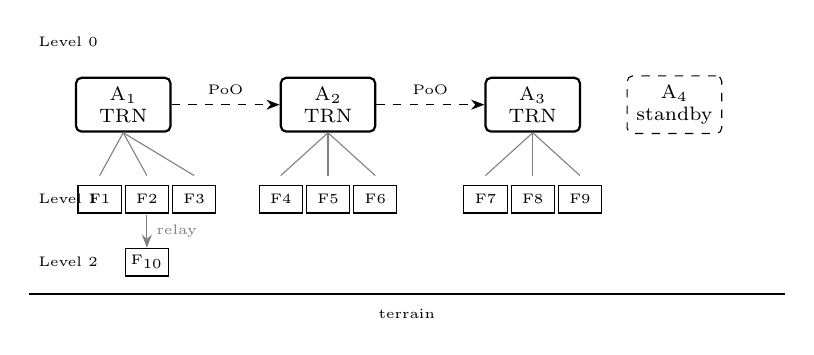
\begin{tikzpicture}[
    anchorbox/.style={draw, thick, rectangle, rounded corners=2pt, minimum width=1.2cm, minimum height=0.6cm, font=\scriptsize, align=center},
    follower/.style={draw, rectangle, minimum width=0.55cm, minimum height=0.35cm, font=\tiny, inner sep=1pt, align=center},
    standby/.style={draw, dashed, rectangle, rounded corners=2pt, minimum width=1.2cm, minimum height=0.6cm, font=\scriptsize, align=center}
]
    \node[anchorbox] (A1) at (0,2.2) {A$_1$\\TRN};
    \node[anchorbox] (A2) at (2.6,2.2) {A$_2$\\TRN};
    \node[anchorbox] (A3) at (5.2,2.2) {A$_3$\\TRN};
    \node[standby] (A4) at (7.0,2.2) {A$_4$\\standby};

    \draw[dashed,->,>=Stealth] (A1) -- node[above,font=\tiny]{PoO} (A2);
    \draw[dashed,->,>=Stealth] (A2) -- node[above,font=\tiny]{PoO} (A3);

    \foreach \x/\n in {-0.3/F1, 0.3/F2, 0.9/F3} {
        \node[follower] at (\x, 1.0) {\n};
        \draw[-,gray] (A1.south) -- (\x, 1.3);
    }
    \foreach \x/\n in {2.0/F4, 2.6/F5, 3.2/F6} {
        \node[follower] at (\x, 1.0) {\n};
        \draw[-,gray] (A2.south) -- (\x, 1.3);
    }
    \foreach \x/\n in {4.6/F7, 5.2/F8, 5.8/F9} {
        \node[follower] at (\x, 1.0) {\n};
        \draw[-,gray] (A3.south) -- (\x, 1.3);
    }

    \node[follower] (FR) at (0.3, 0.2) {F$_{10}$};
    \draw[->,>=Stealth,gray] (0.3, 0.8) -- (FR) node[midway,right,font=\tiny]{relay};

    \draw[thick] (-1.2,-0.2) -- (8.4,-0.2);
    \node[font=\tiny] at (3.6,-0.45) {terrain};

    \node[font=\tiny,anchor=west] at (-1.2,3.0) {Level 0};
    \node[font=\tiny,anchor=west] at (-1.2,1.0) {Level 1};
    \node[font=\tiny,anchor=west] at (-1.2,0.2) {Level 2};
\end{tikzpicture}%
}
\caption{Hierarchical architecture. Active anchors perform mutual Visual Proof of Observation (PoO) between one another and broadcast signed positions over UWB. Followers (Level~1) receive reputation-weighted position directly; deeper followers (Level~2+) receive relayed positions with per-hop noise growth. Standby anchors remain TRN-capable but are not currently elected.}
\label{fig:arch}
\end{figure}

\subsection{System Architecture Overview}

Each UAV runs a common navigation module with four components: a \emph{navigation core} performing visual-inertial odometry (VIO) at 50~Hz and TRN at 0.1~Hz (TRN only on anchors), fused in a local factor graph; an \emph{observation recorder} that produces Signed Observations on each TRN fix; a \emph{mesh protocol handler} managing signed-observation exchange, reputation tracking, and Byzantine rejection; and an \emph{autopilot adapter} layer. The hierarchical topology overlays an anchor/follower structure on this substrate (Fig.~\ref{fig:arch}): anchors perform PoO verification mutually, while followers receive reputation-weighted position via UWB relay with up to $K_\text{max}$ hops.

\subsection{Visual Proof of Observation}

On each TRN fix at position $\mathbf{p}_i \in \mathbb{R}^3$ at time $t_1$, UAV $v_i$ extracts $N=50$ top-scoring feature descriptors $\mathbf{f}_i \in \mathbb{R}^{N\times D}$ ($D{=}256$ for SuperPoint). $N=50$ is a working default: SuperPoint typically yields 200--500 keypoints per image~\cite{detone2018superpoint}; retaining the top-50 by score balances descriptor packet size (50 descriptors at 256 bytes each $= 12.8$\,kB) against matching distinctiveness. Sensitivity to $N$ is deferred to Track~2. The descriptor set forms the hash
\begin{equation}
H_i = \mathrm{SHA\text{-}256}\!\left(\mathrm{sort}_\downarrow(\mathbf{f}_i[0\!:\!N])\right).
\end{equation}
It constructs the Signed Observation
\begin{equation}
\mathrm{OBS}_i = \left(t_1, \mathbf{p}_i, H_i, c_i, \mathrm{ID}_i, \sigma_i\right),
\end{equation}
where $c_i$ is the RANSAC inlier ratio and
\begin{equation}
\sigma_i = \mathrm{Ed25519.sign}\!\left(\mathrm{sk}_i,\, t_1 \Vert \mathbf{p}_i \Vert H_i \Vert c_i \Vert \mathrm{ID}_i\right).
\end{equation}
The base record (Mode~B) totals approximately 180--200~bytes: $t_1$ (timestamp, 8\,B) + $\mathbf{p}_i$ (position $\langle$lat, lon, alt$\rangle$ as three doubles, 24\,B) + $H_i$ (SHA-256 hash, 32\,B) + $c_i$ (RANSAC inlier ratio as a float, 4\,B) + $\mathrm{ID}_i$ (UAV identifier, 8\,B) + $\sigma_i$ (Ed25519 signature, 64\,B) $= 140$\,B core payload, plus message framing (type byte, length, sequence number, CRC, padding) accounting for the remaining 40--60\,B. A \emph{Mode~A} variant appends a compact feature set of $K=20$ descriptors. The value $K=20$ is the minimum that keeps Mode-A packet overhead within budget: $20 \times 256 = 5120$\,bytes $= 5.12$\,kibibytes (KiB) $\approx 5.12$\,kB (binary convention) $= 5.120$\,kB (SI convention, $10^3$-byte base), within the UAV datalink budget assumed in Section~II, bringing total size to $\approx 5.30$\,kB (5120\,bytes of descriptors plus the $\sim$180-byte base record). Ed25519~\cite{bernstein2012ed25519} signature computation is well within sub-millisecond on modern processors at the cycle counts reported by~\cite{bernstein2012ed25519} (84932 cycles for signing); typical ARM Cortex-class embedded targets fall in the same regime, with cycle-exact timings to be characterised on the target board in Track~2.

On receiving $\mathrm{OBS}_i$, a neighbour $v_j$ first verifies $\sigma_i$ using $\mathrm{pk}_i$. If the signature is invalid, reputation $R_i$ is decreased by a signature penalty $\alpha_\text{sig} = 0.30$, a working default equal to $2 \times \alpha_\text{neg} = 0.30$ so a single signature mismatch has the same net reputation impact as two consecutive failed verifications. At a later time $t_2 > t_1$, when $v_j$ flies within verification radius $r_\text{verify} = 500$\,m of $\mathbf{p}_i$, it extracts local features $\mathbf{f}_j$ and computes a verification score. The value $r_\text{verify} = 500$\,m matches the upper end of the UWB operational range (200--500\,m at the datalink power levels assumed in Section~II), ensuring that any follower within UWB communication range can request verification without requiring out-of-range RF links. In \emph{Mode~A} (compact feature set), for each transmitted descriptor, the nearest neighbour in $\mathbf{f}_j$ is accepted if its $L_2$ distance is below $\tau_\text{match} = 0.7$ (Lowe's ratio test threshold~\cite{lowe2004distinctive}: a threshold of 0.7 is the standard lower bound of the accepted range 0.7--0.8 for filtering ambiguous matches, used here with SuperPoint's 256-dimensional $L_2$-normalised descriptors~\cite{detone2018superpoint}); the score $V$ is the ratio of accepted matches to transmitted descriptors, and VERIFIED is declared when $V > T_\text{verify} = 0.3$. The threshold $T_\text{verify}=0.3$ corresponds to $6/20$ Mode-A descriptors (or $6/N$ hash matches in Mode~B) successfully passing the $\tau_\text{match}=0.7$ Lowe-ratio test. Published cross-view SuperPoint matching studies report inlier ratios of 60--90\% under clean line-of-sight conditions, falling to 20--40\% under moderate viewpoint or illumination drift. Setting $T_\text{verify}=0.3$ places the VERIFIED boundary at the lower end of the degraded-but-viable regime, so legitimate verifications continue to pass during moderate environmental noise while complete-failure cases (match ratios below $\sim$20\%, characteristic of wrong-terrain or fabricated-hash submissions from a peer that has not physically observed the claimed region) are reliably rejected. The threshold interacts with $\tau_\text{match}$ and $N,K$: tightening any of the three has the same qualitative effect of raising the false-reject rate against environmentally-degraded honest verifications. Sensitivity over $T_\text{verify}\in\{0.2, 0.3, 0.4\}$ is deferred to Track~2. Because $T_\text{verify}=0.3$ sits at the lower end of the degraded-but-viable regime (20--40\% inlier ratios), honest peers operating under moderate environmental degradation can routinely produce match scores near the exclusion boundary; combined with the asymmetric reputation rule (UNVERIFIED penalty $\alpha_\text{neg}=0.15$), this implies that as few as $\lceil(R_\text{init}-T_\text{reject})/(\alpha_\text{neg}\, R_k)\rceil=2$ consecutive boundary-case UNVERIFIED verdicts under $R_k\!\approx\!1$ would drive an honest peer's reputation to $T_\text{reject}$. A formal false-acceptance / false-rejection (FAR/FRR) characterisation under realistic illumination, viewpoint, and seasonal terrain variation is required to confirm the threshold choice and is part of the Track~2 calibration plan; the corresponding empirical false-exclusion rate is also reported in Limitations (Section~\ref{sec:discussion}). A \emph{Mode~B} variant (hash-only, zero-bandwidth verification) compares recomputed hashes directly; Mode~B is suited to severely bandwidth-constrained tactical deployments in which flight conditions permit reproducible descriptor extraction, and requires additional calibration against the observation geometry (see Section~\ref{sec:discussion}).

The unforgeability rationale is physical: terrain feature descriptors are functions of the surface geometry, illumination, viewing angle, and the learned extractor. A captured UAV cannot fabricate descriptors for a location it has not physically observed without either possessing the imagery database and extractor (which still requires knowledge of the exact atmospheric and illumination conditions at $t_1$) or compromising honest peers before they verify---neither of which is feasible under our threat model. PoO is related to but distinct from the proof-of-location (PoL) literature: PoL systems such as VRChain~\cite{rahouti2022vrchain} (blockchain-anchored visual homing) and BFT-PoLoc~\cite{sheng2024bftpoloc} (Byzantine-fortified trigonometric proof of location from Internet round-trip delays) verify a device's \emph{current} claimed position via either ledger consensus or signal-timing measurements. Visual PoO instead verifies a \emph{past} observation through a neighbour's later physical revisit, with evidence bound to terrain geometry via the learned extractor rather than to network timing or co-located witnesses.

\subsection{Asymmetric Reputation System}
\label{sec:asymmetric-reputation-system}

Each UAV maintains a reputation vector $\mathbf{R} = (R_1,\dots,R_n)$ with $R_j \in [0,1]$ initialised to $R_\text{init} = 0.5$ (neutral prior). The initial reputation is set to the midpoint of the $[0,1]$ range, representing maximum uncertainty about an unknown peer: neither trusted nor distrusted. This is the standard uninformative prior for reputation systems~\cite{josang2007survey}. Updates on verification events are asymmetric:
\begin{align}
\text{VERIFIED: }& R_j \leftarrow \mathrm{clamp}(R_j + \alpha_\text{pos}\, R_k,\, 0, 1), \\
\text{UNVERIFIED: }& R_j \leftarrow \mathrm{clamp}(R_j - \alpha_\text{neg}\, R_k,\, 0, 1), \\
\text{INVALID SIG: }& R_j \leftarrow \mathrm{clamp}(R_j - \alpha_\text{sig},\, 0, 1),
\end{align}
where $R_k$ is the reputation of the verifier. We require $\alpha_\text{neg} \geq 2\alpha_\text{pos}$, preferably $\alpha_\text{neg} \geq 3\alpha_\text{pos}$; the default values are $\alpha_\text{pos} = 0.05$, $\alpha_\text{neg} = 0.15$. The 3:1 ratio ($\alpha_\text{neg}/\alpha_\text{pos}$) is set in Section~\ref{sec:time-byz-exclusion}; the absolute level is anchored by the convergence bound of Proposition~3: to achieve $T_\text{ind} \approx 170$\,s with $R_\text{init}=0.5$, $T_\text{reject}=0.2$, and $\nu_\text{verify}^{-1}\approx45$\,s, the approximation requires $\alpha_\text{neg} \cdot \bar{R}_\text{honest} \cdot \nu_\text{verify} \geq (R_\text{init}-T_\text{reject})/T_\text{ind} \approx 0.30/170 \approx 0.0018$ per second, or $\alpha_\text{neg} \geq 0.0018 \times 45 \approx 0.08$ per verification event; $\alpha_\text{neg}=0.15$ satisfies this with a $\approx 2\times$ margin. The value $\alpha_\text{pos}=0.05$ follows from the 3:1 ratio. Under this asymmetry, three failed verifications outweigh nine successful ones ($3\cdot 0.15 = 9\cdot 0.05 = 0.45$), guaranteeing that distrust accumulates faster than trust while retaining a margin of 2--8 consecutive environment-induced failures before an honest peer is falsely excluded (2 pure-burst events from $R_\text{init}=0.5$ at $R_k=1.0$; up to 8 interleaved VERIFIED+UNVERIFIED rounds from $R_j=1.0$; derivation follows). Let $R_j$ be the \emph{target} peer's current reputation and $R_k$ the \emph{verifier}'s reputation weight. Each UNVERIFIED event decrements $R_j$ by $\alpha_\text{neg} \times R_k$; each VERIFIED event increments $R_j$ by $\alpha_\text{pos}$. For pure-UNVERIFIED bursts (worst case), events needed to drive $R_j$ to $T_\text{reject}=0.2$ are $\lceil(R_j - T_\text{reject})/(\alpha_\text{neg}\times R_k)\rceil$. At $R_k=1.0$ and $R_j=R_\text{init}=0.5$: $\lceil 0.3/0.15\rceil=2$; at $R_j=1.0$: $\lceil 0.8/0.15\rceil=6$. For interleaved sequences (one VERIFIED plus one UNVERIFIED per round), net loss per round is $\alpha_\text{neg}\times R_k - \alpha_\text{pos}$; at $R_k=1.0$, $0.15-0.05=0.10$, giving 3~rounds from $R_j=0.5$ to 8~rounds from $R_j=1.0$. Overall margin: 2 (pure burst from $R_\text{init}$) to 8 (interleaved from $R_j=1.0$) consecutive failures.

To handle dynamic environments, we apply a temporal decay
\begin{equation}
V_\text{weighted} = V \cdot \exp(-\lambda \Delta t),
\end{equation}
with $\lambda = 10^{-3}$~s$^{-1}$ (half-life $\approx$11.5~min). The decay constant is chosen so that an observation becomes effectively stale ($<5\%$ residual weight) after $\approx 3$ half-lives $=34.5$\,min, approximately one-tenth of the 2-hour mission (the one-tenth fraction is an operationally discretionary design goal: it ensures that any single mission phase does not permanently dominate the reputation estimate, while still allowing short-horizon events to decay within one mission); a temporary gap of one revisit cycle ($\nu_\text{verify}^{-1}\approx 45$\,s) causes only $\approx 4.4\%$ decay per missed event ($e^{-10^{-3}\times 45}\approx 0.956$). These are working defaults pending Track~2 sensitivity analysis. Observations older than $T_\text{max\_verify} = 3600$\,s (1\,hour) are considered stale. This cutoff is set to half the 2-hour planned mission length, ensuring that observations from the first half of a mission are discarded before the second half begins. For shorter or longer missions the cutoff should be scaled proportionally.

\subsection{Reputation-Weighted Distributed Factor Graph}

Each UAV maintains a local factor graph $\mathcal{G}_i$ whose maximum-a-posteriori estimate is
\begin{equation}
\mathbf{X}_i^* = \arg\min_{\mathbf{X}} \sum_k \lVert h_k(\mathbf{X}) - \mathbf{z}_k \rVert^2_{\Sigma_k}.
\end{equation}
Three classes of factors are instantiated:
\begin{itemize}
    \item \emph{Local factors} (IMU preintegration~\cite{forster2017preintegration}, VIO, TRN-absolute on anchors, barometric altitude), standard in the art.
    \item \emph{Ranging factors} for each UWB measurement $d_{ij}$ with $h_\text{range}(\mathbf{X}_i, \mathbf{X}_j) = \lVert \mathbf{p}_i - \mathbf{p}_j \rVert_2$, $\sigma_\text{range} = 0.1$~m.
    \item \emph{Reputation-weighted priors} from the Distilled State of neighbour $j$, where the \emph{Distilled State} of UAV~$j$ is the per-UAV broadcast tuple $\mathrm{DS}_j = (t, \mathbf{p}_j, \mathbf{v}_j, \mathrm{cov}(\mathbf{p}_j), R_j, \mathrm{ID}_j, \sigma_j^{\mathrm{Ed25519}})$ comprising timestamp, position, velocity, position-covariance summary, current reputation, identifier, and Ed25519 signature; the byte-level payload composition and bandwidth accounting are given in Section~\ref{sec:theory}-D. The Distilled State is the central inter-UAV communication primitive of the architecture and is consumed by the reputation-prior factor here, by the failover watchdog (Section~\ref{sec:approach}-F, phase F1), and by the load-balancing broadcast (Section~\ref{sec:approach}-G). The reputation-prior factor uses the position $\mathbf{p}_j$ and covariance $\mathrm{cov}(\mathbf{p}_j)$ of $\mathrm{DS}_j$, scaled by $R_j$, with noise
    \begin{equation}
    \sigma_j = \sigma_\text{base} / (R_j + \varepsilon),
    \label{eq:noise_rep}
    \end{equation}
    $\sigma_\text{base} = 50$~m, $\varepsilon = 0.01$ (dimensionless numerical regularisation; chosen two orders of magnitude below $\sigma_\text{base}=50$\,m so $\varepsilon/\sigma_\text{base}=0.02\%$, ensuring negligible influence on the computed covariance). Covariance $\Sigma_j = \mathrm{diag}(\sigma_j^2, \sigma_j^2, (\sigma_j/2)^2)$ for (lat, lon, alt); the halved altitude term reflects a standard anisotropy assumption that UAV barometric altimeters provide tighter altitude bounds than UWB-derived lateral uncertainty. Experiment~1 will characterise whether the actual altitude/lateral ratio differs from 1:2. Sensitivity to $\sigma_\text{base}$: the analytical CEP bound in Proposition~3 scales linearly with $\sigma_\text{base}$; doubling to 100\,m would require approximately $2\times$ as many anchor observations to converge to the 100\,m CEP pass criterion. A full sensitivity sweep over $\sigma_\text{base} \in \{25, 50, 75, 100\}$\,m is planned in Track~2.
\end{itemize}
A UAV with $R = 1.0$ contributes $\sigma \approx 49.5$~m, versus $\sigma \approx 238$~m at $R = 0.2$---approximately a 5$\times$ weight ratio in precision and $\sim$23$\times$ in variance. Optimisation uses iSAM2 with the Bayes-tree representation; the $<$50~ms per-update latency on an embedded accelerator is a design target consistent with published GTSAM/iSAM2 benchmarks~\cite{kaess2012isam2}. The $<$50~ms budget covers the iSAM2 optimisation step only; the full PoO pipeline (camera capture $\sim$10~ms, SuperPoint inference $\sim$20--40~ms on a 50--100~TOPS-class accelerator at 480$\times$640 resolution per published embedded benchmarks~\cite{detone2018superpoint}, top-$N$ sort $<$1~ms, SHA-256 hash $<$1~ms, and Ed25519 signing $<$1~ms at the 84\,932-cycle figure from~\cite{bernstein2012ed25519} on an ARM Cortex-class core) is constrained by the 0.1~Hz TRN fix rate ($=$10~s budget) rather than by the 50~ms factor-graph cycle, so SuperPoint inference timing is not on the critical sub-50~ms path. Per-board characterisation of the PoO pipeline on the specific target accelerator is a Track~2 calibration item; the 50--100~TOPS class is named here as a representative envelope rather than a specific SKU.%

A UWB consistency check provides a secondary, non-visual channel: if UAV $j$ reports position $\mathbf{p}_j^\text{rep}$ but UWB ranging $d_{ij}$ yields $\bigl| \lVert \mathbf{p}_i - \mathbf{p}_j^\text{rep} \rVert - d_{ij} \bigr| > \delta_\text{consist} = 50$\,m, reputation decreases by $\alpha_\text{range} = 0.10$. The threshold $\delta_\text{consist} = 50$\,m matches $\sigma_\text{base}=50$\,m (the declared prior noise), so a consistency check flags deviations beyond one prior standard deviation. The coincidence with $T_\text{spoof}=50$\,m is deliberate: both thresholds are calibrated to the same noise floor. The range-failure penalty $\alpha_\text{range} = 0.10$ is set as the midpoint $(\alpha_\text{pos}+\alpha_\text{neg})/2$, treating a UWB consistency failure as more severe than a single missed verification ($\alpha_\text{pos}$) but less severe than a full failed verification ($\alpha_\text{neg}$), since range failures may arise from temporary link degradation rather than deliberate Byzantine behaviour.

\subsection{Dynamic Anchor Selection and Position Relay}

TRN-capable UAVs compete for anchor status through the score
\begin{equation}
A_i = w_\text{rep} R_i + w_\text{conf} C_i + w_\text{sat} S_i + w_\text{fol} F_i,
\label{eq:anchor_score}
\end{equation}
with default weights $(0.4, 0.3, 0.2, 0.1)$. The weight ordering $w_\text{rep} > w_\text{conf} > w_\text{sat} > w_\text{fol}$ reflects a safety-first hierarchy: trustworthiness must dominate performance, which in turn dominates location-dependent factors (imagery quality varies with where the UAV currently is, not what it is), with load balancing as the lowest-priority factor since over-loading is a soft degradation rather than a safety violation. Placing $w_\text{rep}=0.4$ as the dominant term ensures that a compromised peer with degraded reputation $R_i\to 0$ contributes at most $0.6$ to its anchor score even with maximal $C_i, S_i, F_i$, leaving it below honest candidates whose $R_i\geq T_\text{quorum}=0.6$ adds at least $0.24$ from the reputation term alone---an inherent score gap that makes Byzantine-anchor promotion infeasible without first restoring reputation through honest verifications. Given the strict ordering and the unit-sum constraint $\sum w = 1$, the equal-spacing choice $(0.4, 0.3, 0.2, 0.1)$ is adopted as a working default: the strict weight ordering $w_\text{rep} > w_\text{conf} > w_\text{sat} > w_\text{fol}$ reflects the safety-first hierarchy, the unit-sum constraint $\sum w = 1$ is met by construction, and the choice is deferred to the Track~2 ablation sweep. The spacing $\Delta w = 0.1$ also exceeds the per-event reputation step $\alpha_\text{pos}=0.05$, ensuring that single-verification reputation jitter cannot swap adjacent priority terms in the score ordering. Sensitivity to the weight vector is part of the Track~2 ablation sweep over $w_\text{rep}\in[0.3, 0.5]$, $w_\text{conf}\in[0.2, 0.35]$, $w_\text{sat}\in[0.15, 0.30]$, $w_\text{fol}\in[0.05, 0.20]$ subject to the unit-sum constraint. Here $C_i$ is the TRN confidence (RANSAC inlier ratio), $S_i$ is the imagery coverage quality for the terrain below $v_i$, and $F_i$ is an inverse load factor. Every $T_\text{election} = 60$\,s, the $M$ vehicles with the highest $A_i$ are confirmed as active anchors; a standby replaces an active anchor when its score exceeds the incumbent's by a hysteresis $H = 0.1$. The election period $T_\text{election}=60$\,s is set to exceed the verification revisit cycle ($\nu_\text{verify}^{-1}\approx 45$\,s) by 33\%, allowing at least one full verification round to complete between elections; this prevents frequent re-elections from disrupting ongoing verifications while remaining responsive to anchor degradation. The hysteresis band $H=0.1$ corresponds to two consecutive $\alpha_\text{pos}=0.05$ upward reputation steps, requiring the score gap to represent at least two successful-verification equivalents before triggering a handover. Handover proceeds in three steps (\emph{PROMOTION}, \emph{DEMOTION}, linear-blend) over $T_\text{handover} = 10$~s. $T_\text{handover}=10$\,s matches the failover total budget of Section~\ref{sec:approach}-F (F1--F5 phases sum to $\approx 8$\,s nominal, 10\,s with 5\% packet loss): all anchor-change operations---whether triggered by destruction (failover) or by score-based replacement (planned handover)---share the same architectural timescale, which simplifies the operator's deployment-time reasoning about transition windows. The lower bound on $T_\text{handover}$ is set by the cumulative protocol latency of the three-step PROMOTION $\to$ DEMOTION $\to$ linear-blend sequence (UWB neighbour discovery $\sim 1$\,s, role-change acknowledgement round-trip $\sim 1$--$2$\,s, follower-side covariance update propagation through the iSAM2 factor graph $\sim 1$\,s), so $T_\text{handover}$ must comfortably exceed $\sim 4$\,s to ensure all followers complete their re-association within the blend window. The upper bound is set by the verification revisit cycle: $T_\text{handover}$ must remain well below $\nu_\text{verify}^{-1}\approx 45$\,s so that handovers are decisive on a timescale shorter than reputation reassessment. The value 10\,s sits an order of magnitude below verification cycle and comfortably above protocol latencies. During the blend, both incumbent and standby publish Distilled State updates with time-weighted weights summing to unity; a longer blend would extend this dual-publishing window, increasing UWB neighbour bandwidth consumption and creating more state-merge events at follower-side factor graphs, while a shorter blend risks discontinuities in follower position estimates between the demoted-incumbent's last publication and the promoted-standby's first authoritative state. Sybil protection requires $T_\text{warmup} = 6$ successful verifications before anchor eligibility; at $\nu_\text{verify}^{-1}\approx 45$\,s per cycle, this corresponds to $6\times 45=270$\,s ($\approx 4.5$\,min) of observed honest behaviour, exceeding four full election periods, so a freshly-joining Byzantine peer cannot accumulate quorum influence within a single election cycle. These are working defaults.

\begin{table}[t]
\caption{Consolidated system hyperparameters. Derivation column indicates whether the value is literature-derived (L), operationally discretionary (O), or a working default pending sensitivity analysis (W).}
\label{tab:hyperparams}
\centering
\footnotesize
\setlength{\tabcolsep}{3pt}
\resizebox{\columnwidth}{!}{%
\begin{tabular}{llll}
\toprule
Parameter & Value & Symbol & Derivation \\
\midrule
Feature descriptors per PoO & 50 & $N$ & W \\
Mode-A compact set size & 20 & $K$ & W \\
Signature penalty & 0.30 & $\alpha_\text{sig}$ & W \\
Verification radius & 500\,m & $r_\text{verify}$ & W \\
L2 match threshold & 0.7 & $\tau_\text{match}$ & L (SuperPoint) \\
VERIFIED score threshold & 0.3 & $T_\text{verify}$ & W \\
Initial reputation & 0.5 & $R_\text{init}$ & W \\
Positive reputation step & 0.05 & $\alpha_\text{pos}$ & W \\
Negative reputation step & 0.15 & $\alpha_\text{neg}$ & W (3:1 ratio) \\
Temporal decay constant & $10^{-3}$\,s$^{-1}$ & $\lambda$ & W \\
Staleness cutoff & 3600\,s & $T_\text{max\_verify}$ & O \\
Base prior noise & 50\,m & $\sigma_\text{base}$ & W \\
Noise floor & 0.01 & $\varepsilon$ & W \\
UWB consistency threshold & 50\,m & $\delta_\text{consist}$ & W \\
Range-failure penalty & 0.10 & $\alpha_\text{range}$ & W \\
Anchor-score weights & (0.4,0.3,0.2,0.1) & $w_{1..4}$ & W \\
Election period & 60\,s & $T_\text{election}$ & O \\
Standby-replace hysteresis & 0.10 & $H$ & W \\
Handover blend duration & 10\,s & $T_\text{handover}$ & O \\
Sybil warmup count & 6 & $T_\text{warmup}$ & W \\
Per-hop noise growth & 0.15 & $\beta$ & W \\
Max relay hops (ISR) & 3 & $K_\text{max}$ & O \\
Max relay hops (patrol) & 5 & $K_\text{max}$ & O \\
Reject threshold & 0.20 & $T_\text{reject}$ & W \\
Quorum reputation floor & 0.60 & $T_\text{quorum}$ & W \\
Load-balance period & 30\,s & $T_\text{balance}$ & O \\
Load-balance low threshold & 30\% & $P_\text{low}$ & O \\
Load-balance high threshold & 150\% & $P_\text{high}$ & O \\
Spoof position threshold & 50\,m & $T_\text{spoof}$ & W \\
Consecutive spoof count & 3 & $N_\text{consecutive}$ & W \\
Mass-spoofing trigger & 30\% & $P_\text{mass}$ & O \\
\bottomrule
\end{tabular}%
}
\end{table}

Followers compute their position as the reputation-weighted average
\begin{equation}
\mathbf{p}_\text{fol} = \frac{\sum_j w_j\, \mathbf{p}_j}{\sum_j w_j}, \quad w_j = \frac{R_j}{\sigma_{\text{hop},j}^2},
\label{eq:fusion}
\end{equation}
where for a $k$-hop relay chain,
\begin{equation}
\sigma_k = \sigma_\text{anchor}\, (1 + \beta)^k,
\label{eq:hop}
\end{equation}
with $\beta = 0.15$ per hop (per-hop noise growth factor, a conservative working default; see Section~III discussion) and $\sigma_\text{anchor}$ given by~(\ref{eq:noise_rep}). The multiplicative form $\sigma_k = \sigma_\text{anchor}(1+\beta)^k$ models two physical effects that compound at each relay hop in a UWB-trilaterated position chain: (i) additive UWB ranging-measurement variance $\sigma_\text{range}^2$ from the new measurement to the previous hop, and (ii) propagated upstream position uncertainty from the previous hop's estimate, weighted by a Geometric Dilution of Precision (GDOP) factor that depends on the local anchor configuration. Under perfectly independent ranging and ideal anchor geometry, error propagation is sublinear (\emph{additive variance model}): $\sigma_k = \sqrt{\sigma_\text{anchor}^2 + k\sigma_\text{range}^2}$, growing as $\sqrt{k}$ for large $k$---this is the theoretical lower bound for independent Gaussian ranging noise. The multiplicative form is not a physical prediction but a \emph{conservative engineering bound}: it dominates the additive model for all $k \geq 1$ when $\beta > 0$, as $(1+\beta)^k > \sqrt{1 + k(\sigma_\text{range}/\sigma_\text{anchor})^2}$ for typical UWB parameters. Under correlated upstream uncertainty or poor geometry (anchors nearly collinear with the follower), GDOP amplifies propagated variance beyond the sublinear baseline, with the worst case approaching exponential $(1+\beta)^k$ growth. The multiplicative form is therefore the \emph{conservative} engineering bound for the planned non-collinear but topologically constrained swarm. The value $\beta = 0.15$ is adopted as a conservative working default for the per-hop standard-deviation growth factor; it represents a 15\% std-dev increase per hop relative to the prior hop, chosen as a round figure within the typical range expected for UWB cross-trilateration under benign (line-of-sight) propagation and pending empirical refit against a measured UWB NLOS dataset in Track~2. From this $\beta$, the $K_\text{max}=3$ ISR ceiling follows as a derived quantity (at the reference operating point $\sigma_\text{anchor}\approx 58$\,m, $R_\text{anchor}=0.85$, $\sigma_3 \approx 88$\,m, giving single-anchor CEP$_{50}=1.177\sigma_3 \approx 104$\,m, slightly exceeding the 100-m NATO-grade target by $\approx 4\%$; under multi-anchor reputation-weighted fusion ($m{=}2$--$3$) the bound improves to CEP$_{50}\in[60,74]$\,m, comfortably within the target); $K_\text{max}=3$ is not used to motivate the choice of $\beta$. A sensitivity sweep over $\beta \in \{0.05, 0.10, 0.15, 0.20\}$ is planned in Track~2 and will shift the derived $K_\text{max}$ accordingly. The functional form and value of $\beta$ are subject to empirical refit in Track~2: if measured $\sigma_k$ versus $k$ fits a sublinear $\sqrt{k}$ form or a different multiplicative rate $\beta'$ better than the conservative $(1+0.15)^k$ assumption, the bound in Proposition~\ref{prop:conv} relaxes accordingly without affecting the analytical structure. The base noise $\sigma_\text{base}$ is a configurable system parameter; we adopt $\sigma_\text{base} = 50$~m for consistency across the experiments reported below, with other values applicable to swarm configurations that assume different baseline anchor accuracy. For a well-performing anchor with $R_\text{anchor} = 0.85$, $\sigma_\text{anchor} = 50/0.86 \approx 58.1$~m; propagation yields $\sigma_1 \approx 66.8$, $\sigma_2 \approx 76.9$, $\sigma_3 \approx 88.4$, and $\sigma_5 \approx 116.9$~m. The 5-hop value exceeds the 100-m target both as $\sigma_5$ and as the corresponding CEP$_{50}\approx 138$\,m; for NATO-grade ISR we therefore recommend $K_\text{max}=3$ under the default multi-anchor fusion regime, reserving $K_\text{max}=5$ for lower-precision patrol missions. The patrol value $K_\text{max}=5$ is reported as an upper operational envelope, not a precision recommendation: at $R_\text{anchor}=0.85$ the per-hop derivation yields $\sigma_5 \approx 117$\,m (CEP$_{50}\approx 138$\,m), exceeding the 100\,m NATO-grade ISR target. The intermediate $K_\text{max}=4$ is not separately reported because it is not operationally distinct from $K_\text{max}=5$ for precision purposes; $K_\text{max}=3$ under multi-anchor fusion is the maximum strictly ISR-compliant depth (single-anchor at $k=3$ exceeds the CEP target by $\approx 4\%$ and is flagged for deployment-time review). The patrol use case accepts precision on the order of $\sim 150$\,m CEP or coarser in exchange for a $1.67\times$ greater effective swarm reach (relay radius $2.5$\,km at $K_\text{max}=5$ versus $1.5$\,km at $K_\text{max}=3$, given the 500-m UWB hop range). For anchors operating below the reference $R_\text{anchor}=0.85$, $\sigma_k$ scales as $1/(R_\text{anchor}+\varepsilon)$ per~(\ref{eq:noise_rep}), so both bounds tighten proportionally; the precision tolerance is a per-mission operator decision and the relay-depth ceiling is set deployment-time as a function of the mission's precision class. If $R_\text{anchor}$ drops from $0.85$ to $0.30$, $\sigma_\text{anchor}$ rises to $\sim$161~m and all downstream followers automatically receive degraded weights through~(\ref{eq:fusion}) without any explicit control signal: \emph{reputation flows down the hierarchy through noise covariance}.

\begin{figure}[t]
\centering
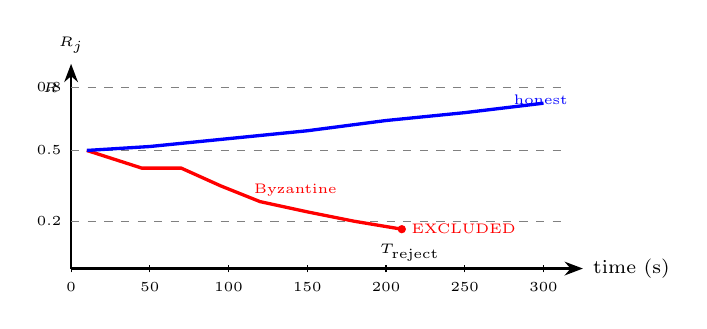
\begin{tikzpicture}[font=\scriptsize, >=Stealth]
    \draw[->,thick] (0,0) -- (6.5,0) node[right]{time (s)};
    \draw[->,thick] (0,0) -- (0,2.6) node[above,font=\tiny]{$R_j$};
    \foreach \y/\lab in {0.6/0.2, 1.5/0.5, 2.3/0.8} {
        \draw[gray,dashed] (0,\y) -- (6.3,\y);
        \node[anchor=east,font=\tiny] at (0,\y) {\lab};
    }
    \node[font=\tiny,anchor=east] at (-0.05,2.3) {$R$};
    \foreach \x/\lab in {0/0, 1/50, 2/100, 3/150, 4/200, 5/250, 6/300} {
        \draw (\x,-0.05) -- (\x,0.05);
        \node[font=\tiny,anchor=north] at (\x,-0.05) {\lab};
    }
    \draw[red,very thick] plot coordinates {(0.2,1.5) (0.9,1.275) (1.4,1.275) (1.9,1.05) (2.4,0.85) (3.0,0.72) (3.6,0.6) (4.2,0.5)};
    \node[red,anchor=west,font=\tiny] at (4.2,0.5) {EXCLUDED};
    \fill[red] (4.2,0.5) circle (1.5pt);
    \draw[blue,very thick] plot coordinates {(0.2,1.5) (1.0,1.55) (2.0,1.65) (3.0,1.75) (4.0,1.88) (5.0,1.98) (6.0,2.1)};
    \node[blue,anchor=west,font=\tiny] at (5.5,2.15) {honest};
    \node[red,anchor=west,font=\tiny] at (2.2,1.0) {Byzantine};
    \node[font=\tiny,anchor=west] at (3.8,0.2) {$T_\text{reject}$};
\end{tikzpicture}
\caption{Schematic of the analytically predicted reputation trajectory under a na\"ive Byzantine attack (Section~\ref{sec:sim}-C; empirical validation deferred). The compromised UAV's reputation decays after each failed Proof-of-Observation verification while honest peers continue to accumulate trust. Permanent exclusion is predicted within the worst-case upper bound $T_\text{exclusion}\lesssim 215$~s (Proposition~\ref{prop:conv}); the schematic marks $T\!\approx\!210$~s, at which three independent honest verifiers have each driven $R_j$ below $T_\text{reject}=0.2$. The per-step drop $R_4: 0.5\to 0.425$ illustrated at $T{=}45$~s corresponds to an illustrative verifier weight $R_k=0.5$ (so that $\alpha_\text{neg}\cdot R_k = 0.075$); the operational deployment uses $R_k$ drawn from the honest reputation distribution, and the Proposition~\ref{prop:conv} bound uses the conservative substitution $R_k\to\bar{R}_\text{honest}=0.53$ for the analytical estimate.}
\label{fig:repu}
\end{figure}

\subsection{Automatic Failover Protocol}

Anchor loss (destruction, jamming, or reputation falling below $T_\text{reject}$) triggers a five-phase protocol executing within 10~s:
\begin{itemize}
    \item \textbf{F1 Detection} (0--5~s): a watchdog declares anchor unavailability after $T_\text{timeout} = 5$~s without a DistilledState message. During the timeout, orphaned followers propagate by IMU dead reckoning, accumulating $<$5~m drift at 30~m/s.
    \item \textbf{F2 REASSIGN\_REQUEST} (5--6~s): each orphaned follower broadcasts its device ID, last known position, velocity, battery state, and sensor capabilities.
    \item \textbf{F3 REASSIGN\_OFFER} (6--7~s): surviving anchors respond with their ID, position, reputation, and available capacity.
    \item \textbf{F4 Selection} (7--8~s): the follower computes
    \begin{equation}
    S_\text{reassign} = \alpha_\text{prox}/d + \alpha_\text{rep} R + \alpha_\text{cap}(1 - L),
    \label{eq:reassign}
    \end{equation}
    with defaults $(0.4, 0.35, 0.25)$.
    \item \textbf{F5 Attachment} (8--10~s): ATTACH/ATTACH\_ACK exchanges position and covariance.
\end{itemize}
\begin{figure}[t]
\centering
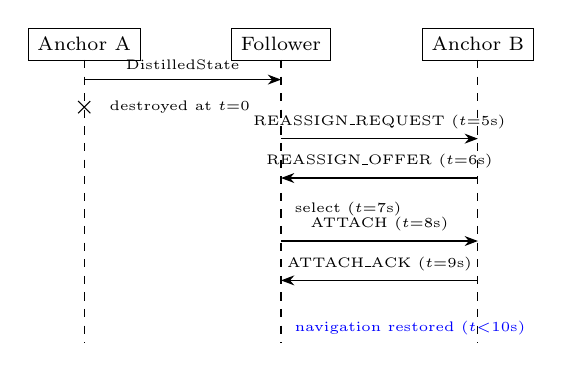
\begin{tikzpicture}[font=\scriptsize, >=Stealth, node distance=0.1cm]
    \node[draw, minimum width=1.2cm, minimum height=0.35cm] (AA) at (0,3.0) {Anchor A};
    \node[draw, minimum width=1.2cm, minimum height=0.35cm] (FF) at (2.5,3.0) {Follower};
    \node[draw, minimum width=1.2cm, minimum height=0.35cm] (AB) at (5.0,3.0) {Anchor B};
    \foreach \x in {0,2.5,5.0} \draw[dashed] (\x,2.8) -- (\x,-0.8);

    \draw[->] (0,2.55) -- node[above,font=\tiny]{DistilledState} (2.5,2.55);
    \node[font=\tiny,cross out,draw,minimum size=4pt,inner sep=0] at (0,2.2) {};
    \node[font=\tiny,anchor=west] at (0.2,2.2) {destroyed at $t{=}0$};

    \draw[->] (2.5,1.8) -- node[above,font=\tiny]{REASSIGN\_REQUEST ($t{=}5$s)} (5.0,1.8);
    \draw[<-] (2.5,1.3) -- node[above,font=\tiny]{REASSIGN\_OFFER ($t{=}6$s)} (5.0,1.3);
    \node[font=\tiny,anchor=west] at (2.55,0.9) {select ($t{=}7$s)};
    \draw[->] (2.5,0.5) -- node[above,font=\tiny]{ATTACH ($t{=}8$s)} (5.0,0.5);
    \draw[<-] (2.5,0.0) -- node[above,font=\tiny]{ATTACH\_ACK ($t{=}9$s)} (5.0,0.0);
    \node[font=\tiny,anchor=west,text=blue] at (2.55,-0.6) {navigation restored ($t{<}10$s)};
\end{tikzpicture}
\caption{Failover sequence upon anchor destruction. Dead-reckoning drift during the 5-second timeout is $<$5~m at 30~m/s cruise speed.}
\label{fig:failover}
\end{figure}
Byzantine rejection proper removes all factors of UAV $j$ from the local graph when $R_j < T_\text{reject} = 0.2$; permanent exclusion additionally requires $M$ independent UAVs, each with $R > T_\text{quorum} = 0.6$, to confirm the exclusion. From Proposition~3, convergence is predicted at $T_\text{ind} = (R_\text{init}-T_\text{reject})/(\alpha_\text{neg}\,\bar{R}_\text{honest}\,\nu_\text{verify}) \approx 170$\,s; with $R_\text{init}=0.5$ the gap $R_\text{init}-T_\text{reject}=0.3$ drives the numerator. A smaller $T_\text{reject}$ would increase convergence time, while a larger $T_\text{reject}$ would increase false exclusions of honest peers; $T_\text{reject}=0.2$ keeps the honest-peer safety margin above 2 environment-induced failures at $R_k=0.5$ (see Proposition~1 analysis). The quorum reputation floor $T_\text{quorum}=0.6$ requires a verifier to have earned at least two successful verifications above the initial state ($T_\text{quorum} = R_\text{init} + 2\alpha_\text{pos} = 0.5 + 0.10 = 0.6$), so a freshly-joined peer cannot self-confirm into the quorum; the minimum defensible value is $T_\text{quorum} > R_\text{init} = 0.5$, and $T_\text{quorum}=0.6$ provides a minimal earned-trust barrier. Coincidentally $T_\text{quorum} = 3 \times T_\text{reject}$, but the binding constraint is the margin above $R_\text{init}$, not the factor of $3$; the factor of $3$ is a working default providing a clear separation between verifier quality and exclusion threshold. The default $M = 3$ tolerates $f \leq M-1 = 2$ colluding Byzantine peers irrespective of $n$; safety for larger $f$ requires $M$ to scale with $f$, as analysed in Section~\ref{sec:theory}. Fig.~\ref{fig:failover} summarises the timing.

\subsection{Load Balancing and GNSS Spoofing Detection}

Every $T_\text{balance} = 30$\,s, anchors broadcast a STATUS field (appended to the standard Distilled State message of Section~\ref{sec:approach}-D) including their follower count. The load-balancing period is set to one-half of the election period ($T_\text{election}=60$\,s), allowing two load-balance checks per election cycle; at $\nu_\text{verify}^{-1}\approx 45$\,s, a 30\,s check interval falls between consecutive verifications. The target is $T_\text{target} = N_\text{total}/N_\text{anchors}$. If an anchor's count is below $P_\text{low} T_\text{target}$ (30\%) or above $P_\text{high} T_\text{target}$ (150\%), a redistribution protocol (TRANSFER\_OFFER $\rightarrow$ TRANSFER\_ACCEPT $\rightarrow$ REASSIGN\_COMMAND $\rightarrow$ smooth linear-blend handover over $T_\text{handover} = 10$~s) transfers followers from overloaded to underloaded anchors. The asymmetric band reflects the asymmetric cost of under- vs over-loading: an overloaded anchor ($>150\%$ of target) risks queue overflow and message drops, while an underloaded anchor ($<30\%$ of target) wastes TRN capacity without causing message loss. Overload headroom: $P_\text{high}-1.0=0.50$; underload floor: $1.0-P_\text{low}=0.70$. These are working defaults consistent with general load-balancing practice~\cite{eager1986adaptive}.

GNSS-spoofing detection operates at 1~Hz on each UAV that still has a GNSS receiver (relevant when GNSS is only partially denied or during the transition into full-denial operation). The vehicle compares its GNSS-reported position with a UWB-trilaterated position from at least three neighbours with $R > T_\text{min}$, where $T_\text{min} = T_\text{reject} = 0.20$ excludes peers that are already excluded by the reputation system from participating in the consistency cross-check. If $\lVert \mathbf{p}_\text{GNSS} - \mathbf{p}_\text{UWB} \rVert > T_\text{spoof} = 50$\,m for $N_\text{consecutive} = 3$ successive measurements, GNSS is marked unreliable and the affected vehicle falls back to reputation-weighted UWB position. The spoofing detection threshold is set equal to $\sigma_\text{base}=50$\,m so that UWB-measured positions deviating from the claimed GNSS position by more than one prior standard deviation are flagged as anomalous; UWB ranging error at 500\,m range is typically 10--30\,cm (1-$\sigma$), so $T_\text{spoof}=50$\,m corresponds to $\sim$170--500$\,\sigma_\text{UWB}$, far above any legitimate ranging uncertainty. $N_\text{consecutive}=3$ requires three consecutive exceedances, reducing false-positive rate to approximately $p^3$ where $p$ is the per-sample false-alarm rate; three is the minimum count providing a causal chain (removes single-sample noise artefacts) while remaining below the $T_\text{warmup}=6$ threshold (so an attacker cannot ``pass'' warmup before being flagged). When the proportion of spoofed UAVs exceeds $P_\text{mass} = 30\%$, the entire swarm transitions to a \emph{full GNSS-denial mode}: GNSS is disabled globally and the swarm relies exclusively on TRN anchors with UWB relay. This mass-spoofing threshold is set well above the per-Proposition-1 maximum Byzantine fraction ($f/n \leq 2/200 = 1\%$ under default $M=3, f=2$): a coordinated attack on 30\% of the swarm constitutes a scenario outside the individual-exclusion threat model, where full-GNSS-denial mode is the appropriate response. The 30\% figure is chosen just below the classical Byzantine bound $f<1/3\approx 33\%$: when $>30\%$ of the swarm reports spoofed positions, the collective deviation exceeds the Byzantine-fault-tolerant range of the reputation mechanism (which tolerates $f<M-1$ individual colluders, not 30\% of 200 UAVs simultaneously), so global GNSS-denial mode is the appropriate response. This is a working default, operator-configurable. By design, GNSS spoofing does not affect navigation reputation $R_i$; only failed Proof-of-Observation verifications decrement reputation, so a UAV spoofed by an external emitter is not punished for an attack it did not launch.

\section{Theoretical Analysis}
\label{sec:theory}

\subsection{Quorum Safety}
\label{sec:quorum-safety}

\begin{proposition}[Quorum safety against na\"ive Byzantine peers]
\label{prop:safety}
Let $M$ be the permanent-exclusion quorum size. Assume (i)~na\"ive Byzantine peers fail every Proof-of-Observation verification (they claim positions they have not physically observed); (ii)~honest peers correctly issue VERIFIED or UNVERIFIED verdicts; (iii)~each UAV maintains its reputation state $R_j$ locally from its own verifications, without gossip-based propagation of reputation values between peers; and (iv)~the per-peer rate of environment-induced UNVERIFIED verdicts on honest targets, $\rho_\text{env}$ (events per second), satisfies $\rho_\text{env} < \alpha_\text{pos}\, \nu_\text{verify}/\alpha_\text{neg}$, so that honest peers accumulate VERIFIED events faster than environmental penalties drive $R$ toward $T_\text{reject}$. Condition~(iv) is a \emph{rate condition on the environmental failure regime}; the Remark below quantifies what happens when it is violated (e.g., persistent cloud cover or night-time operation). The proposition provides no safety guarantee against environment-induced false exclusion when (iv) is violated, only against deliberate Byzantine attack; and (v)~$R_\text{init} < T_\text{quorum}$, so that a freshly-joined Byzantine peer cannot be self-confirmed into the quorum by virtue of its initial reputation alone (the default values $R_\text{init}=0.5 < T_\text{quorum}=0.6$ satisfy this). If $f \leq M-1$, no set of colluding Byzantine peers can trigger false permanent exclusion of an honest UAV.
\end{proposition}

\begin{IEEEproof}[Sketch]
Permanent exclusion requires $M$ independent UAVs, each with $R > T_\text{quorum}$, to declare the target $R_j < T_\text{reject}$. Na\"ive Byzantine peers cannot raise their reputation above $T_\text{quorum}$ because every verification attempt against them yields UNVERIFIED (assumption~(i)); each UAV tracks this locally from its own verifications without reputation gossip (assumption~(iii)), so collusion to inflate a Byzantine peer's remote reputation is blocked; and the initial reputation $R_\text{init} < T_\text{quorum}$ (assumption~(v)) ensures no freshly-joined peer enters the quorum immediately. Therefore any false quorum contains at most $f$ Byzantine members; if $f < M$, at least one honest member would need to declare a false UNVERIFIED on an honest target, which contradicts assumption~(ii). Assumption~(iv) further ensures that an honest target's reputation does not drift below $T_\text{reject}$ from environmental causes alone, eliminating the alternative failure mode of false exclusion driven by accumulated environment-induced UNVERIFIED events.
\end{IEEEproof}

\begin{remark}
If Assumption~(iv) is violated (e.g., dense cloud cover or night-time operation rendering terrain features undetectable so $\rho_\text{env}$ rises sharply), Proposition~\ref{prop:safety} still holds against deliberate Byzantine attack but does not prevent environment-induced false exclusion of an otherwise-honest UAV. In that operational regime, operator intervention or automatic mode switch to INS-only localisation is required.
\end{remark}

\begin{proposition}[Parameter scaling]
\label{prop:scaling}
Assume $n \geq M + f + 1$. Then the default configuration $M=3$ tolerates at most $f=2$ colluding Byzantine peers. The precondition $n \geq M+f+1$ ensures that $M$ honest verifiers can always be assembled independently of the $f$ Byzantine nodes, with one additional honest peer as a reserve against transient communication failure; the formal mathematical minimum is $n \geq M + f$ (the quorum can be exactly filled by honest peers with none to spare), but at this boundary any single transient unavailability blocks quorum assembly, so $n \geq M+f+1$ is the recommended operational floor. For $M=3$, $f=2$ this gives $n \geq 6$. At $n=5$, only $5-f=3$ honest peers remain, which exactly meets $M=3$ but leaves no spare verifier; any additional failure violates the constraint. The precondition $n \geq M+f+1$ must be enforced by the deployment operator. For swarms that require tolerance of more adversaries, $M$ must be configured as $M \geq f+1$, subject to the further constraint that at least $M$ honest peers must accumulate $R > T_\text{quorum}$ before exclusion becomes possible.
\end{proposition}

The classical Byzantine impossibility bound $f < \lfloor (n-1)/3 \rfloor$~\cite{lamport1982byzantine} (with related graph-theoretic robustness conditions developed by~\cite{leblanc2013resilient} for the W-MSR setting) is \emph{achievable} in our system---but only if $M$ is scaled accordingly; it is not automatic from swarm size. This is a design trade-off: a small $M$ gives fast exclusion in small swarms, a large $M$ gives stronger guarantees in large swarms at the cost of slower exclusion times.

\textbf{Strategic adversaries.} Proposition~\ref{prop:safety} assumes na\"ive Byzantine behaviour. Strategic Byzantine adversaries---which the trust-based multi-agent literature has long recognised as difficult~\cite{yemini2022characterizing,mallmanntrenn2022crowd}---can in principle maintain $R > T_\text{quorum}$ between observable attacks. Our system provides partial mitigation through (i)~the UWB consistency check (Section~\ref{sec:approach}-D), which catches range--position inconsistencies independent of PoO; (ii)~the asymmetric reputation rule, which amplifies any single failed verification; and (iii)~the temporal-decay mechanism, which prevents historical trust from indefinitely shielding an adversary. A formal treatment of strategic Byzantine resilience is beyond the scope of this paper and is left to future work.

\subsection{Time to Na\"ive Byzantine Exclusion}
\label{sec:time-byz-exclusion}

\begin{proposition}[Convergence bound]
\label{prop:conv}
Assume (i)~$R_j = R_\text{init}$ at the moment the target $j$ begins Byzantine behaviour (i.e.\ the bound applies at the moment of compromise, before any honest-trust accumulation; if $j$ has accumulated $R_j > R_\text{init}$ during a warm-up window of duration $T_\text{warmup}$, the bound increases proportionally to $(R_j - T_\text{reject})/(R_\text{init} - T_\text{reject})$, replacing the numerator of Eq.~(\ref{eq:tind})); and (ii)~the per-event verifier reputation weight is approximated by its honest-equilibrium value $R_k \approx \bar{R}_\text{honest}$ (the substitution $R_k \leftarrow \bar{R}_\text{honest}$ in Eqs.~(1)--(3) collapses the per-event modulation to a constant drift coefficient). Let $\nu_\text{verify}$ denote the mean rate (in s$^{-1}$) at which honest UAVs fly over regions claimed by a Byzantine peer, and let $\bar{R}_\text{honest}$ be the average honest reputation. (The verification \emph{radius} $r_\text{verify}=500$\,m of Section~\ref{sec:approach}-B is a distinct quantity.) For a na\"ive Byzantine peer, the expected time at a single honest verifier to drive $R_j$ below $T_\text{reject}$ is
\begin{equation}
T_\text{ind} \approx \frac{R_\text{init} - T_\text{reject}}{\alpha_\text{neg}\, \bar{R}_\text{honest}\, \nu_\text{verify}}.
\label{eq:tind}
\end{equation}
Permanent exclusion additionally requires $M$ independent honest verifiers to reach the threshold. Because the verifier set is not strictly independent---different verifiers may overlap on the same claimed region and start their verification sequences at correlated times---the additional quorum delay is bounded below by $(\rho-1)/\nu_\text{verify}$, where $\rho\geq 1$ captures inter-verifier overlap. A closed-form expression for $\rho$ in realistic topologies is beyond the scope of this paper; empirical characterisation of the quorum delay is the purpose of Experiment 3 of the proposed evaluation methodology (Section~\ref{sec:sim}).
\end{proposition}

Substituting representative parameter choices $R_\text{init}=0.5$, $T_\text{reject}=0.2$, $\alpha_\text{neg}=0.15$, and the design assumptions $\bar{R}_\text{honest}=0.53 \approx R_\text{init} + 0.5\alpha_\text{pos} = 0.5 + 0.025 = 0.525$ (one half-step above the initial state; a conservative lower estimate bounded between $R_\text{init}=0.5$ and $\approx 0.6$; the actual equilibrium via the temporal-decay ODE is deferred to Track~2; a higher equilibrium would yield faster exclusion) and $\nu_\text{verify}^{-1}\approx 45$~s (design input; corridor-geometry lower bound: anchor traversal of one coverage cell diameter $2r_\text{verify}=1000$\,m at $v_p=30$\,m/s takes $1000/30 \approx 33$\,s; the additional $\approx 12$\,s is a conservative overhead budget for UWB handshake round-trip ($\lesssim 2$\,s), TRN fix latency ($\lesssim 5$\,s at 0.1~Hz fix rate), and scheduling jitter ($\lesssim 5$\,s); exact characterisation deferred to Track~2) give $T_\text{ind}\approx 170$~s. A closed-form geometric derivation of $\nu_\text{verify}^{-1}$ depends strongly on the specific anchor routing pattern; a tractable analytical model is left to future work. Adding the inter-verifier quorum delay $(\rho-1)/\nu_\text{verify}$ under the working assumption $\rho \leq 2$ (i.e.\ inter-verifier overlap adds at most one additional verification interval at the $M=3$ default, consistent with the patrol-topology revisit cycle of Section~\ref{sec:sim}-A) and noting that $T_\text{ind}$ is reported in seconds via $\nu_\text{verify}$ in s$^{-1}$ (whereas the simulator's per-cell $T_\epsilon$ is reported in rounds, with one round corresponding to one observation step in the abstract simulator), yields an analytical \emph{estimated worst-case upper bound} $T_\text{exclusion}\lesssim 215$~s under these conservative parameter substitutions; the actual exclusion time is expected to be lower whenever the operational equilibrium $\bar{R}_\text{honest} > 0.53$ holds (e.g., $\bar{R}_\text{honest}\to 1$ in the high-trust limit gives $T_\text{ind} \approx 90$\,s and $T_\text{exclusion}\lesssim 135$\,s). Empirical characterisation of the actual exclusion-time distribution relative to this worst-case bound is the purpose of Experiment~3 of the proposed evaluation methodology (Section~\ref{sec:sim}-C).

\subsection{Multi-Hop Error Propagation}

From~(\ref{eq:hop}), the $k$-hop standard deviation satisfies $\sigma_k = \sigma_\text{anchor}(1+\beta)^k$. The mean-squared error of the fused position~(\ref{eq:fusion}) at a follower receiving $m$ anchor contributions with weights $w_j$ is
\begin{equation}
\mathrm{MSE} = \frac{\sum_j w_j^2 \sigma_j^2}{\left(\sum_j w_j\right)^2},
\end{equation}
which follows directly from the standard weighted-average variance identity for independent Gaussian observations~\cite{kay1993estimation}. The independence assumption is only approximate in the deployed system: multiple anchor position estimates are jointly maintained inside a shared iSAM2 Bayes-tree factor graph and share UWB-ranging factors, so their residual covariances are partially correlated; the MSE expression above is therefore an \emph{optimistic} (lower-bound) estimate of the achievable CEP under reputation-weighted fusion. The empirical CEP measured in Experiment~1 of Section~\ref{sec:sim} will be the binding deployment number; the analytical bound is reported here for design-time parameter selection.
For $\sigma_\text{anchor}=58.1$~m (i.e., $R=0.85$, $\sigma_\text{base}=50$~m) and $\beta=0.15$, the corresponding CEP$_{50}=1.177\sigma_k$ for the single-anchor case crosses the 100-m NATO threshold between $k=2$ (CEP$\approx 90$\,m) and $k=3$ (CEP$\approx 104$\,m, $\approx 4\%$ over); under default multi-anchor fusion ($m{=}2$--$3$), the bound at $k=3$ improves to CEP$\in[60,74]$\,m, well within the target. Our recommendation $K_\text{max}{=}3$ is therefore predicated on the multi-anchor fusion regime that is the system's default operating mode; single-anchor relay at $k=3$ is marginally non-compliant and should be flagged at deployment time.

\subsection{Communication Complexity}

Each UAV broadcasts a Distilled State message at 1~Hz, totalling approximately 185~bytes. The payload composition is: position $\langle$lat, lon, alt$\rangle$ as three doubles (24~B), velocity $\langle v_x, v_y, v_z\rangle$ as three floats (12~B), $3{\times}3$ symmetric covariance summary (6 floats $=$ 24~B), timestamp (8~B), UAV identifier (8~B), compact reputation/state-flag block (20~B), Ed25519 signature (64~B), and framing overhead (type byte, length, sequence number, CRC, padding $\approx$25~B), summing to $\approx 185$~B. For a typical UWB neighbourhood of $n_\text{local}\approx 10$ UAVs (within $\sim$100\,m range, not the full $n=200$ swarm), each vehicle receives $n_\text{local}-1 = 9$ inbound messages per second, giving an inbound bandwidth of $9 \times 185~\text{B} \times 8~\text{bit/B} \times 1~\text{Hz} \approx 13.3$~kbit/s. A Signed Observation ($\sim$180--200~B; see Section~\ref{sec:approach}-B) is transmitted only on TRN fixes at 0.1\,Hz, adding negligible overhead. No consensus round-trip is required in the critical navigation path, distinguishing our approach from blockchain-based schemes whose route-commitment finality is on the order of seconds per round, a property of the blockchain settlement layer~\cite{strobel2020blockchain,strobel2023robot}. Signal-processing approaches for single-UAV spoofing detection (e.g., deep CNN-BiLSTM frameworks~\cite{badar2025deepspoofnet}) do not address cooperative swarm-wide verification and therefore do not replace the cross-peer architecture proposed here.

\section{Proposed Evaluation Methodology}
\label{sec:sim}

This section specifies the simulation methodology designed to validate the analytical predictions of Section~\ref{sec:theory}. The methodology has not yet been executed: empirical results are deferred to future work in a Gazebo/ROS2-based framework currently under development. Each experiment below states (i)~the configuration, (ii)~the metric of interest, (iii)~the analytical prediction (where the theory provides one), and (iv)~the pass criterion. Reporting the planned methodology in this paper rather than ad-hoc post-hoc results is intentional: it pre-registers what the proposed system would measure and how a fair comparison against prior art could be conducted.

\subsection{Planned Evaluation Setup}

The intended scenario is a swarm of $n=200$ UAVs over a $200\times 200$~km rural corridor at 300~m altitude and 30~m/s cruise speed: five UAVs TRN-capable (active anchors), two TRN-capable standby, and the remaining 193 followers. Coverage is achieved via a mobile-anchor patrol model rather than static deployment~\cite{he2003rangefree}: each anchor sweeps the corridor, providing follower updates at a revisit rate of $\nu_\text{verify}^{-1}\approx 45$\,s. The operative coverage metric is the maximum revisit interval experienced by any follower, not instantaneous geometric overlap; at any instant, 5 anchors at 500\,m UWB range cover $5\pi(0.5)^2\approx 4$\,km$^2$ of the 40\,000\,km$^2$ corridor ($\approx 0.01\%$), which is sufficient because followers receive periodic updates during anchor sweeps rather than requiring continuous line-of-sight coverage. The anchor count of five is a design input: with $K_\text{max}=3$ relay hops and a per-hop range of 500\,m, the maximum relay radius is $3 \times 500 = 1500$\,m, so a single anchor can serve followers within this radius at any instant; two standby anchors provide redundancy against single-point anchor failure as required by Experiment~2. At any instant, $K_\text{max}=3$ relay hops give a single-anchor coverage footprint of $\pi(1.5)^2\approx 7$\,km$^2$ and five anchors a combined $\approx 35$\,km$^2$, i.e.\ $\approx 0.09\%$ of the $40{,}000$\,km$^2$ corridor; full corridor coverage therefore requires that the union of the five anchors' patrol routes intersects every follower's position within the revisit cycle $\nu_\text{verify}^{-1}\approx 45$\,s. The specific patrol-route geometry that achieves this (e.g., evenly-spaced longitudinal sweeps, lawnmower partitions, or an outer-loop / inner-loop split between active and standby anchors) is a deployment-time decision treated as out of scope here; the analytical scenario assumes the followers are distributed such that the above revisit condition is met by construction, and Track~2 will validate this against a concrete patrol-route schedule. GNSS is fully denied in the default setup (the spoofing experiment uses a partial-GNSS configuration, see Experiment~4). Planned terrain imagery is Sentinel-2 at 10\,m GSD (bands B2, B3, B4); Sentinel-2 is the standard open-access satellite imagery source for large-area TRN research~\cite{drusch2012sentinel} and its 10\,m multispectral bands (290\,km swath, 5-day revisit at high latitudes) provide sufficient resolution for the SuperPoint feature-extraction pipeline at the corridor scale. Higher-resolution commercial sources (e.g., 0.5\,m imagery) are not used because their licensing restrictions and per-tile cost are incompatible with the open research framing of this paper. Sensor noise parameters of the planned simulator are: MEMS-grade IMU (10~$^\circ$/h drift), UWB $\pm$0.1\,m, TRN CEP $\sim$35\,m, barometric altitude $\pm$2~m\,(MEMS barometric altimeter working default; MEMS barometers typically specify $\pm$1--3~m absolute accuracy at room temperature; Track~2 hardware selection will pin the specific sensor datasheet). Planned mission duration: 2 hours per run. The intended implementation is a Python/C++ simulator with iSAM2 (GTSAM~4.2)~\cite{kaess2012isam2}. iSAM2 is chosen over batch solvers (g2o, Ceres) and sliding-window SAM because its Bayes-tree incremental update mechanism provides amortised $O(\log n)$ complexity per new measurement by updating only the affected portion of the factor graph; batch solvers would require a full re-linearisation sweep on each update, which does not scale to 200 nodes at 45-second intervals. Each experiment is to be repeated with 25 Monte Carlo seeds (seed values $s_i = i$ for $i \in \{1, 2, \ldots, 25\}$, using the NumPy default random generator with \texttt{numpy.random.default\_rng($s_i$)}) for statistical characterisation; the seed count is chosen to give a standard error of the mean within roughly 5\% of typical metric magnitudes under the assumption of seed-independent Gaussian noise, and will be adjusted upward in the actual run if observed variance is larger.

The planned simulation stack (Python orchestration layer interfacing a C\texttt{++}/GTSAM~4.2 back-end) is expected to require on the order of 2~hours wall-clock time per seed on a modern workstation-class CPU (e.g., 8-core, 3.5\,GHz), yielding approximately $25 \times 6 \approx 150$ core-hours for the full evaluation suite. These estimates are provisional and will be refined once the Track~2 simulation framework is implemented; the Section~V pass criteria do not depend on achieving any particular runtime.

\textbf{SwarmRaft baseline (planned comparison).} The intended comparison is against an author reimplementation of SwarmRaft~\cite{dev2025swarmraft} configured with author-chosen parameters (5-peer leader group, 10-s leader re-election period, median-based position correction); these parameters are not specified in the original SwarmRaft paper. The values are working defaults selected to match the conservative end of the Raft consensus parameter space~\cite{ongaro2014raft}: Raft's original evaluation used election timeouts of 150--300\,ms for LAN deployments; we scale to 10\,s to account for the higher latency of long-range UAV RF links and to ensure leader stability across the $\nu_\text{verify}^{-1} \approx 45$\,s verification cycle. The 5-peer group is the minimum Raft quorum size ($\lfloor 5/2 \rfloor + 1 = 3$ for majority) that provides two-fault tolerance. These parameters are subject to sensitivity analysis in Track~2. The same UWB/TRN sensor-noise model is used for the baseline as for the proposed system. Because SwarmRaft does not maintain persistent reputation across rounds, ``time-to-exclusion'' for the baseline is to be measured as the wall-clock time at which the fraction of rounds in which a target peer's report is overruled by the median exceeds 90\% for ten consecutive elections---a functional analogue of exclusion. Other reasonable definitions yield similar ordering. A head-to-head comparison against the original SwarmRaft codebase remains future work.

\subsection{Proposed Experiment 1: CEP vs.\ Relay Depth}

\textbf{Configuration}: nominal honest-peer operation with $\sigma_\text{base}=50$\,m; reputation-weighted fusion across $m = 2$--$3$ anchors per follower typical of the planned topology (see~(\ref{eq:fusion})). The value $\sigma_\text{base}=50$\,m is set as a conservative prior slightly exceeding the TRN CEP specification of $\sim$35\,m: a 50\,m Gaussian $1\sigma$ corresponds to CEP $\approx 50 \times 1.177 \approx 59$\,m (using the CEP$\approx 1.177\sigma$ relation for a circular normal distribution), providing a starting prior that the iSAM2 smoother contracts as observations accumulate. Sensitivity to $\sigma_\text{base}$ is deferred to Track~2.
\textbf{Metric}: CEP at each relay level $k \in \{0,1,2,3,5\}$, min--max across 25 seeds. Level $k=4$ is omitted as it provides no qualitatively distinct operating regime between $k=3$ (ISR ceiling) and $k=5$ (patrol ceiling); the chosen set brackets each $K_\text{max}$ with one level on each side of the transition.
\textbf{Analytical prediction}: Table~\ref{tab:cep_predicted} gives the CEP$_{50}$ ranges derived from~(\ref{eq:fusion})--(\ref{eq:hop}) with $\beta=0.15$, using the standard CEP$_{50}=1.177\sigma_k$ relation for a 2D circular Gaussian; lower bounds assume $m=3$-anchor reputation-weighted fusion and upper bounds the single-anchor case, with $\sqrt{m}$ scaling between them. Inter-seed variance bounds will be reported alongside the empirical CEP in Track~2.
\textbf{Pass criterion}: under the default multi-anchor fusion configuration ($m=2$--$3$), levels up to $k{=}3$ remain under the 100-m NATO threshold across all 25 seeds (Table~\ref{tab:cep_predicted} predicts $\leq 74$~m at $k=3$ for $m=2$); $k{=}5$ exceeds the threshold in the high-percentile tail, confirming the theoretical analysis of Section~\ref{sec:theory}-C. Single-anchor relay at $k=3$ is marginally non-compliant (CEP$\approx 104$~m, $\approx 4\%$ over) and is reported separately as a worst-case bound rather than the operational target. On this basis the architecture specifies $K_\text{max}{=}3$ for ISR missions and reports $K_\text{max}{=}5$ only as an upper operational envelope. An INS-only dead-reckoning baseline is expected to reach the kilometre scale over a 2-hour mission given the MEMS-grade IMU drift, against which the relay scheme is predicted to yield more than an order-of-magnitude reduction.

\begin{table}[t]
\centering
\caption{Analytical CEP prediction vs.\ Relay Hop Count, with $\sigma_\text{base}{=}50$~m, $R_\text{anchor}=0.85$ ($\sigma_\text{anchor}\approx 58.1$~m), and $\beta=0.15$. Bounds are computed via the standard CEP$_{50}=1.177\sigma_k$ relation for a 2D circular Gaussian; lower bounds correspond to $m{=}3$-anchor reputation-weighted fusion (CEP$_{50}\approx 1.177\sigma_k/\sqrt{3}$), upper bounds to the single-anchor case ($m{=}1$). Empirical validation is the purpose of Experiment~1.}
\label{tab:cep_predicted}
\small
\resizebox{\columnwidth}{!}{%
\begin{tabular}{@{}cllc@{}}
\toprule
Level & Role & Position Source & Predicted CEP (m) \\
\midrule
0 & Anchor (TRN) & Cam + imagery + GTSAM & 30--50 \\
1 & Direct follower & Anchor + UWB & 45--79 \\
2 & Relay (2 hops) & Relay + UWB & 52--90 \\
3 & Deep (3 hops) & 2nd relay + UWB & 60--104 \\
5 & Maximum (5 hops) & 5th relay + UWB & 79--138 \\
\bottomrule
\end{tabular}%
}
\end{table}

\subsection{Proposed Experiment 2: Anchor Failover}

\textbf{Configuration}: at $T{=}15$~min, anchor~\#3 (bearing approximately 39 followers given the planned topology) is destroyed by simulated kinetic impact. The trigger time $T=15$\,min is chosen to occur (a) well after the system warmup phase ($T_\text{warmup} \times \nu_\text{verify}^{-1} = 6 \times 45\,\text{s} = 270$\,s $\approx 4.5$\,min; $T=15$\,min is $\approx 3.3\times$ the warmup duration), and (b) past one temporal-decay half-life ($\ln 2/\lambda \approx 11.5$\,min), so anchor~\#3 has accumulated approximately $(15-4.5)/(\nu_\text{verify}^{-1}/60) \approx 14$ post-warmup verification opportunities per verifier-peer and operates in the asymptotic regime of both reputation accumulation and decay---representing the loss of an \emph{established} anchor rather than a recently-promoted candidate. The remaining $120-15=105$\,min provides a long post-failover observation window for characterising swarm CEP recovery after orphan reassignment. Earlier trigger times ($T<10$\,min) would test recently-promoted anchors with non-asymptotic reputation, conflating failover dynamics with bootstrap dynamics; later trigger times would compress the observation window without adding scenario value. The REASSIGN protocol is expected to redistribute orphans across the remaining anchors.
\textbf{Metric}: total switching time (anchor destruction to all-followers-reattached) and maximum dead-reckoning drift during the interval, mean$\pm$std across 25 seeds; same statistics under injected 5\% packet loss. The 5\% packet-loss injection is a working default chosen to match the Experiment~2 analytical-prediction stress regime: ``injecting 5\% packet loss is predicted to push the mean toward but below the 10-s design budget'' (Section~\ref{sec:sim}-B Analytical prediction). The value 5\% therefore tests the failover protocol at the operating point where the design prediction expects a near-budget but in-budget outcome, providing a direct empirical check of the analytical model. The lower edge of the operating envelope is clean line-of-sight UWB (commercial DW3000-class ranging radios report typical loss well below $1\%$ at sub-500-m range under low-mobility conditions); the upper edge is set by the F1--F5 budget itself, beyond which retransmission overhead saturates the 10\,s budget and the test transitions from operating-envelope to failure-mode characterisation. A sensitivity sweep over $\{1\%, 5\%, 10\%, 20\%\}$ is planned in Track~2 to characterise the full envelope; the same sweep will calibrate the packet-loss model against measured airborne UWB link statistics, which the available published literature does not report at the per-link granularity required for direct substitution at this stage.
\textbf{Analytical prediction}: failover phases F1--F5 (Section~\ref{sec:approach}-F) sum to a cumulative latency on the order of 8~s under nominal UWB, with the F1 watchdog interval ($\approx 5$~s) the dominant term; injecting 5\% packet loss is predicted to push the mean toward but below the 10-s design budget.
\textbf{Pass criterion}: total switching time $<10$~s under both nominal and 5\%-packet-loss conditions, with no follower left orphan after the protocol completes; the per-phase intervals are recorded individually so the dominant contributor to any over-budget run can be identified. The ``no orphan'' criterion applies seed-by-seed: in \emph{each} of the 25 seeds, every follower attached to the destroyed anchor must successfully reattach to a surviving anchor within the 10-s budget; partial failures (e.g., one orphan in one seed) constitute a failed pass and trigger investigation. % PRIORITY-5: M2-423-orphan-seed-fraction

\subsection{Proposed Experiment 3: Byzantine Detection and Exclusion}
\label{sec:exp3-byz-detection}

\textbf{Configuration}: at $T{=}10$~s, anchor~\#4 is compromised (na\"ive Byzantine) and begins transmitting Signed Observations with spoofed positions displaced by 2~km. The 2-km spoofed position displacement is a working default chosen to lie well above all detection thresholds and well below the operational-area scale: (a) well above the UWB consistency threshold $\delta_\text{consist}=50$\,m, so the UWB cross-check flags the displacement independently of PoO verification; (b) well above the worst-case per-hop position uncertainty $\sigma_3 \approx 88$\,m at the $K_\text{max}=3$ relay bound (2\,km $\approx 23\,\sigma_3$), so the displacement cannot be washed out by a verifier's own position noise regardless of its hop distance from a trusted reference; (c) well above the TRN CEP of $\sim 35$\,m, ensuring the claimed-terrain region's descriptors differ substantively from those at the anchor's actual location---this is the primary PoO detection path; and (d) well below the 200-km corridor scale (2\,km $= 1\%$ of corridor), so the displaced claimed position remains within the simulated terrain database and within reach of patrolling honest peers who can verify it. Both detection paths (UWB consistency and PoO descriptor mismatch) fire independently at this displacement; values between $\sim 200$\,m and $\sim 5$\,km yield qualitatively identical Byzantine-exclusion behaviour. The specific 2-km value is reported for reproducibility rather than as a derived bound. Sensitivity over $\{100\,\text{m}, 500\,\text{m}, 2\,\text{km}, 10\,\text{km}\}$ is planned in Track~2. Signatures remain valid (key compromised with the UAV), but descriptor hashes do not match the claimed terrain. Note: the compromise trigger at $T=10$\,s precedes the $T_\text{warmup}=6$ successful verifications required for Sybil protection ($6\times \nu_\text{verify}^{-1}\approx 270$\,s). This intentionally tests the pre-warmup worst-case: the analytical bound (Proposition~\ref{prop:conv}) applies with $\bar{R}_\text{honest}$ estimated from $R_\text{init}$, representing maximum attacker advantage at the moment of compromise.
\textbf{Metric}: time from compromise to permanent exclusion ($R_4 < T_\text{reject}$ confirmed by $M{=}3$ independent verifiers), mean$\pm$std across 25 seeds.
\textbf{Analytical prediction}: Section~\ref{sec:theory}-B's worst-case upper-bound estimate $T_\text{exclusion}\lesssim 215$~s under the conservative parameters $R_\text{init}{=}0.5$, $T_\text{reject}{=}0.2$, $\alpha_\text{neg}{=}0.15$, $\bar{R}_\text{honest}=0.53$, $\nu_\text{verify}^{-1}\!\approx\!45$~s.
\textbf{Pass criterion}: empirical mean exclusion time must not exceed the worst-case bound by more than $25\%$, i.e.\ $\bar{T}_\text{empirical} \leq 1.25 \times 215 = 268.75$~s, evaluated on the seed-aggregate mean; lower empirical values are unconstrained and expected whenever the operational $\bar{R}_\text{honest} > 0.53$. The $25\%$ tolerance allows for the inter-verifier correlation factor $\rho$ in Proposition~\ref{prop:conv} (unmodelled analytically) and finite-seed variance. Per-seed exclusion times are reported as a distribution (min, max, mean, std) for transparency, but pass/fail is the aggregate; additionally, the 90th-percentile per-seed exclusion time must not exceed $1.5\times 215 = 322.5$~s, to flag high-variance seeds that would indicate unmodelled inter-verifier correlation not captured in the aggregate mean. % PRIORITY-5: M2-430-bound-seed-fraction
The SwarmRaft baseline (planned reimplementation per Section~\ref{sec:sim}-A) is expected to reach functional exclusion noticeably slower owing to the absence of cross-round reputation accumulation in Raft-family protocols. Fig.~\ref{fig:repu} illustrates the predicted reputation trajectory schematically: at $T{=}45$~s, the first honest UAV flies over the claimed region and computes e.g.\ $V = 0.10$ (illustrative schematic score), dropping $R_4$ from $0.5$ to $0.425$; subsequent honest verifications drive $R_4$ below $T_\text{reject}$, triggering permanent exclusion within the worst-case upper bound $T_\text{exclusion}\lesssim 215$~s (Proposition~\ref{prop:conv}). A formal head-to-head comparison against the original SwarmRaft codebase remains future work (Section~\ref{sec:discussion}-C).

\subsection{Proposed Experiment 4: GNSS Spoofing Reaction}

\textbf{Configuration}: a separate intended setup ($n=50$, partial GNSS denial), distinct from the primary 200-UAV fully-GNSS-denied configuration, to isolate spoofing-detection behaviour in the regime where a GNSS receiver is still available. The $n=50$ size is the minimum that keeps the 10\% spoofed share ($=5$ UAVs) above the $M+f+1=6$ peer feasibility floor of Proposition~\ref{prop:safety}, ensuring at least one honest verifier remains available; it also isolates the spoofing sub-protocol from concurrent anchor-election confounds present at $n=200$. An external spoofer displaces the GNSS solution of 5 UAVs (10\%) by 120~m. The 10\% share is chosen as a moderate partial-swarm attack fraction consistent with the individual-exclusion threat model ($f/n \ll 30\%$); the 120\,m displacement is chosen to be well above the spoofing threshold $T_\text{spoof}=50$\,m while remaining within the 2-km displacement tested in Experiment~3. The 10\% share is chosen as the minimum sub-swarm fraction that keeps the test above the $M+f+1$ quorum floor while remaining below $P_\text{mass}=30\%$; the 120\,m displacement is set to $2.4\times T_\text{spoof}=50$\,m, providing sufficient margin for the $N_\text{consecutive}=3$ detection test to complete (at 1\,Hz sampling, 3 exceedances require 3\,s) before a patrolling honest UAV can close from outside $r_\text{verify}=500$\,m. Both are working defaults subject to sensitivity analysis in Track~2; a sensitivity sweep over $\{50\,\text{m}, 120\,\text{m}, 500\,\text{m}\}$ displacement and $\{5\%, 10\%, 20\%\}$ spoofed share is planned.
\textbf{Metric}: time from spoofing onset to reputation-weighted UWB fallback, mean$\pm$std across 25 seeds; maximum positional deviation during the transition.
\textbf{Analytical prediction}: the UWB cross-check is configured to trigger after 3 consecutive discrepancies (latency $\approx 3$~s at 1~Hz cycle), followed by $\approx 1$~s switching latency, giving an expected reaction time on the order of 4~s; the transient deviation is predicted to be approximately the spoofing displacement (120~m) plus single-step IMU drift.
\textbf{Pass criterion}: reaction time $<5$~s in at least 90\% of seeds, with no propagation of spoofed positions into the swarm-wide factor graph. Reputation is \emph{not} affected (spoofing is external, not a PoO violation), consistent with the design principle of separating spoofing victims from malicious peers. The 10\% spoofed share is chosen as the minimum sub-swarm fraction that keeps the test above the $M+f+1$ quorum floor while remaining below $P_\text{mass}=30\%$; the 120\,m displacement is chosen as $2.4\times T_\text{spoof}=50$\,m (design choice). Both are independent of the specific parameter values in~\cite{mykytyn2023gpsspoofing,bi2024spoofing}, which motivate the threat model rather than the specific test parameters.

\subsection{Proposed Experiment 5: Progressive Attrition}

\textbf{Configuration}: a 2-hour mission with progressive loss of 1 anchor and 44 followers (representing a 22.5\% total attrition: $(1+44)/200 = 22.5\%$) through uniform random attrition, with failure times drawn independently and uniformly from $[0, T_\text{mission}] = [0, 7200]$\,s for each of the 45 lost UAVs. The 22.5\% figure is chosen to stress-test the system near the edge of its designed tolerance: with 7 TRN-capable UAVs (5 active + 2 standby), losing 1 anchor requires promotion of a standby, and the 44-follower loss reduces the relay graph density without dropping below the minimum required for $K_\text{max}=3$ hop paths. The uniform distribution is chosen as the most conservative prior in the absence of an empirical failure-time model; it ensures attrition events are neither clustered (best-case) nor front-loaded (worst-case) but spread across the full mission. At least one mission segment routes an active anchor across an imagery-degraded region (e.g., water, uniform terrain) to exercise automatic standby-anchor promotion.
\textbf{Metric}: count of load-balancing handover triggers; per-handover blend perturbation (defined as the maximum follower-CEP deviation observed during a $T_\text{handover}=10$\,s linear-blend window relative to steady-state CEP immediately before the trigger, reported per handover-event and aggregated as mean$\pm$std across all events across all 25 seeds); aggregate CEP throughout the mission; and any automatic standby promotions (binary event per seed: \emph{at least one} standby promotion triggered during the mission; additionally report the total count of standby promotions per seed as mean$\pm$std across 25 seeds, to characterise load-balancing frequency rather than merely confirming the mechanism triggered at least once). % PRIORITY-5: M1-442-blend-perturbation, M1-442-standby-promotion
\textbf{Analytical prediction}: the load-balancing protocol is expected to trigger on the order of $10$--$20$ times across the 2-hour window given the planned attrition rate, each handover completing within $T_\text{handover}=10$~s with instantaneous perturbation on the order of a few metres; aggregate CEP is expected to stay below the 100-m NATO requirement throughout.
\textbf{Pass criterion}: aggregate CEP $<100$\,m evaluated as the worst-case seed-aggregate (max over the 25 per-seed mission-aggregate CEPs), matching the NATO-grade ISR requirement that the bound be met deterministically across the planned operational envelope; zero orphan-follower episodes in each of the 25 seeds (a follower must not remain detached for more than $T_\text{handover}+T_\text{timeout}=15$\,s after losing its prior anchor), giving a required seed-fraction of 25/25; and at least one successful standby promotion event in each of the 25 seeds when the active anchor traverses the imagery-degraded region. The imagery-degraded region is specified geometrically as a circular patch of 15\,km diameter centred at $(100\,\text{km}, 100\,\text{km})$ in the $200\times 200$\,km corridor, representing terrain over which SuperPoint feature extraction yields fewer than the required $N=50$ keypoints (e.g., uniform water, snow, or low-texture cropland); the active anchor's patrol path is constrained to traverse this patch at least once per mission. % PRIORITY-5: M2-444-CEP-seed-fraction, M2-444-orphan-seed-fraction, M2-444-standby-topology, M3-441-imagery-degraded

\subsection{Proposed Experiment 6: Ablation}

\textbf{Configuration}: four single-pillar disabled variants (no reputation, no PoO, no failover, no load balancing) plus the full system, each run for 25 seeds.
\textbf{Metric}: Byzantine-exclusion time, mean CEP, and post-failure outcome (orphan count or MAC overload), per variant.
\textbf{Analytical prediction} (Table~\ref{tab:ablation_expected}): disabling reputation collapses Byzantine exclusion entirely (the trust-weighted noise covariance is the mechanism of exclusion) and produces order-of-magnitude position-error amplification; disabling PoO leaves cryptographic-signature checking in place but loses the physical-observation tie, allowing valid-signature spoofed positions from a compromised key to pass; disabling failover permanently orphans followers attached to a destroyed anchor; disabling load balancing leads to UWB MAC overload at the most-loaded anchor as attrition progresses.
\textbf{Pass criterion}: each disabled variant exhibits the predicted failure mode in at least 90\% of seeds; the full system is the only configuration meeting all four behavioural requirements simultaneously. MAC overload in the ``no load balancing'' variant is defined as: the surviving most-loaded anchor's UWB transmission queue grows monotonically and exceeds the per-anchor 1\,Hz Distilled-State broadcast budget for any 60-second window during the 2-hour mission; this condition must be observed in $\geq 90\%$ of seeds for the variant and \emph{not} observed in the full-system variant. % PRIORITY-5: M1-449-post-failure-outcome

\begin{table}[t]
\centering
\caption{Ablation: expected qualitative outcomes per disabled pillar, derived from the architecture's design intent. Quantitative validation is the purpose of Experiment~6. ``$\infty$'' denotes complete failure of the corresponding capability.}
\label{tab:ablation_expected}
\small
\setlength{\tabcolsep}{3pt}
\resizebox{\columnwidth}{!}{%
\begin{tabular}{@{}lccc@{}}
\toprule
Variant & Byz.\ excl. & Mean CEP & Post-failure \\
\midrule
Full system        & $\lesssim 215$~s & $\sim$50~m & 0 orphans \\
No reputation      & $\infty$ & severely degraded & 0 orphans \\
No PoO             & $\infty$ & nominal & 0 orphans \\
No failover        & nominal & nominal & $\sim$39 orphans \\
No load balancing  & nominal & nominal & MAC overload\textsuperscript{$\dagger$} \\
\bottomrule
\end{tabular}%
}
\vspace{2pt}
{\scriptsize Cells are analytical predictions (Section~\ref{sec:theory}); empirical validation is the purpose of Experiment~6. ``No reputation'' / ``No PoO'' rows: $\infty$ means the corresponding exclusion mechanism is absent. \textsuperscript{$\dagger$}Expected to exceed UWB medium-access capacity at the most-loaded surviving anchor under continued attrition; no orphan count defined for this failure mode.}
\end{table}

% Computational validation backbone
\input{BFT_UAV_Swarm_Paper_v9_8/sections/uav-asym-decay}
\input{BFT_UAV_Swarm_Paper_v9_8/sections/uav-clamp-convergence}
\input{BFT_UAV_Swarm_Paper_v9_8/sections/uav-byzantine-scaling}

\section{Discussion}
\label{sec:discussion}

\subsection{Limitations}

\textbf{Bootstrap period.} With $R_\text{init}{=}0.5$ and $T_\text{quorum}{=}0.6$, permanent exclusion is not operational until honest peers accumulate sufficient reputation through successful cross-verifications; during this short warm-up the signature-validation layer and UWB-consistency check remain active. Deployments should include a pre-flight cross-verification phase or lower $T_\text{quorum}$ during mission initiation to close this window.

\textbf{Mode~B feasibility.} The hash-only verification variant (Section~\ref{sec:approach}-B) requires reproducible descriptor extraction across UAVs, which in turn requires controlled illumination, viewpoint alignment, and deterministic extractor settings. Mode~B is therefore suited primarily to severely bandwidth-constrained deployments with calibrated observation geometry; Mode~A (compact feature set, $L_2$ matching) is the default for general operation.

\textbf{UWB NLOS.} The $\beta{=}0.15$ per-hop noise growth assumes benign (line-of-sight) propagation. A fully cluttered (non-line-of-sight) deployment would require a measured-NLOS-aware $\beta(k)$; the current model is best interpreted as a rural/line-of-sight baseline, with NLOS calibration deferred to Track~2.

\textbf{Temporal decay.} The $\lambda = 10^{-3}$~s$^{-1}$ decay assumes quasi-static terrain. Active combat zones can alter descriptors on shorter timescales than 11.5~min, motivating a learned adaptive $\lambda$.

\textbf{Re-admission.} The re-admission protocol for previously excluded UAVs was not evaluated. In adversarial settings, an attacker with sustained physical access could repeatedly re-enrol compromised vehicles; mitigations include out-of-band operator authorisation and increasing $T_\text{warmup}$ with re-admission count.

\subsection{Deployment Considerations}

Implementation targets commercial off-the-shelf embedded platforms capable of approximately 50--100~TOPS of inference throughput, standard short-range UWB ranging radios, MEMS- or tactical-grade inertial sensors, and a secure element for Ed25519 key storage. The navigation module integrates without modification of the underlying flight-control firmware (PX4/ArduPilot via MAVLink or proprietary autopilots via Ethernet). Because the follower tier requires no camera, imagery database, or GPU-class accelerator, a large swarm can combine a small number of fully-equipped anchor UAVs with many minimally-equipped followers, yielding a substantial reduction in per-UAV navigation hardware cost at the swarm level.\footnote{A representative bill-of-materials comparison between the anchor and follower profiles is part of the associated patent application and is not reproduced here; a quantitative cost-multiplier figure is deferred to a future deployment-engineering paper where component-level pricing can be reported transparently.}

\subsection{Design-Space Comparison with Prior Art}
\label{sec:comparison}

Table~\ref{tab:comparison} summarises the design-space comparison against the closest published systems, including BFTL~\cite{castelloferrer2022bftl} as the four-pillar prior-art benchmark. The comparison is structured by which of the six target pillars each system supports, and on the qualitative architectural choices (continuous-state estimator vs.\ discretised maps; hardware tested vs.\ simulation-only). Per-metric quantitative entries for the proposed system are deferred to the empirical-validation phase (Section~\ref{sec:sim}); the analytical predictions of Section~\ref{sec:theory} establish the target numerical ranges. The proposed architecture is, to our knowledge, the only published design that simultaneously addresses all six pillars within a continuous-state flight-grade estimator. BFTL is the closest prior art on pillar coverage (BFT, hierarchy, reputation, relay) but operates over \emph{discretised graph-structured environments} with blockchain-settled route commitments on the order of seconds per round, a property of the chosen settlement layer rather than of the BFTL formalism itself~\cite{strobel2020blockchain}; the published instantiation as deployed is consequently incompatible with the 50-ms control cycles required by flight-grade continuous-state estimation. The present architecture adds automatic failover and GNSS-spoofing detection while replacing discretised map commitments with an incremental factor-graph estimator, which is the substantive gap BFTL leaves open.

\begin{table}[t]
\centering
\caption{Design-space coverage of the proposed architecture vs.\ the closest published systems. Pillars: BFT consensus over navigation data, anchor/follower hierarchy, persistent cross-round reputation, automatic anchor-loss failover, GNSS-spoofing detection, multi-hop position relay. The right-most columns capture the architectural choices that gate compatibility with flight-grade control. The proposed system's pillars are design intent; their empirical realisation is the purpose of the experiments in Section~\ref{sec:sim}. Note on BFTL's ``reputation'' pillar credit: in the BFTL formalism~\cite{castelloferrer2022bftl} this entry refers to blockchain-weighted route commitments rather than reputation-weighted noise-covariance modulation of the state estimator (the mechanism in our architecture); the two are distinct technical commitments under the shared ``reputation'' label.}
\label{tab:comparison}
\small
\setlength{\tabcolsep}{3pt}
\resizebox{\columnwidth}{!}{%
\begin{tabular}{@{}lcccc@{}}
\toprule
Pillar / Capability & Ours & SwarmRaft & BDGD & BFTL \\
\midrule
BFT consensus              & \checkmark & ($\sim$)   & \checkmark & \checkmark \\
Anchor/follower hierarchy  & \checkmark & --         & --         & \checkmark \\
Persistent reputation      & \checkmark & --         & \checkmark & \checkmark \\
Automatic failover         & \checkmark & ($\sim$)   & --         & -- \\
GNSS-spoofing detection    & \checkmark & \checkmark & \checkmark & -- \\
Multi-hop position relay   & \checkmark & --         & --         & \checkmark \\
\midrule
Continuous-state est.\     & yes & yes & yes & no \\
Hardware UAVs tested       & no & no & no & no \\
\bottomrule
\end{tabular}%
}
\end{table}

\subsection{Future Work}
\label{sec:futurework}

Five directions stand out. \emph{First}, execution of the proposed evaluation methodology of Section~\ref{sec:sim} in a Gazebo/ROS2-based simulation framework, including the SwarmRaft reimplementation comparison; this is the immediate next milestone. \emph{Second}, hardware validation at 10--20 UAV scale with injected adversarial behaviour, which our systematic review suggests has not yet been reported for BFT-aware UAV navigation. The concurrent Swarm Oracle work~\cite{pacheco2025swarmoracle} demonstrates such validation on 12 ground robots for blockchain-oracle scenarios; extending this validation methodology to GNSS-denied UAV flight is a natural next step. \emph{Third}, a head-to-head comparison against the original SwarmRaft~\cite{dev2025swarmraft} codebase, in addition to the author reimplementation planned in Section~\ref{sec:sim}. \emph{Fourth}, adversarial multi-hop error characterisation---closing a gap flagged explicitly in the BDGD paper~\cite{zhong2025bdgd}. \emph{Fifth}, learned role adaptation using reinforcement-learning schemes such as CI-HRL~\cite{xiang2025cihrl} or semantic coordination as in RALLY~\cite{wang2025rally}, integrated with the Byzantine-resilient substrate presented here.

\subsection*{Code and Data Availability}
Three Monte Carlo simulator implementations supporting the empirical-validation sections (Sections~\ref{sec:asym-decay-empirical}--\ref{sec:byzantine-scaling-empirical}) are released at \url{https://github.com/ok-research/bft-uav-swarm-validation} under the MIT licence; each section's Reproducibility paragraph identifies the corresponding subdirectory and tag. Physics-grounded experiments in a Gazebo/ROS2 simulation environment remain deferred to a forthcoming track and will be released alongside that follow-on work. Sentinel-2 imagery used for Terrain-Referenced Navigation is publicly available through the Copernicus Open Access Hub (\url{https://scihub.copernicus.eu/}) under the Copernicus Data Space open-access licence; no custom dataset is generated by the present code release.

\section{Conclusion}
\label{sec:conclusion}

We presented a Byzantine-fault-tolerant hierarchical navigation architecture for GNSS-denied UAV swarms that integrates, within a continuous-state flight-grade factor-graph estimator, six previously disjoint capabilities: BFT consensus, dynamic anchor/follower hierarchy, reputation-weighted multi-hop position relay, sub-10-second automatic failover by design, UWB-based GNSS-spoofing detection, and load balancing under progressive attrition. A systematic review of approximately 90 publications from 2020--2026 indicates that, to our knowledge, no prior published system has combined more than four of these pillars, and none has done so in a continuous-state flight-grade estimator. The central primitive, visual Proof of Observation, ties trust to terrain-anchored evidence (physically bound to terrain geometry, illumination, and the learned extractor; not forgeable by a vehicle that has not observed the location under the threat model adopted here) and integrates naturally with factor-graph state estimation via asymmetric reputation-weighted noise. Theoretical analysis exposes an explicit trade-off between quorum size and scalable Byzantine tolerance, gives a closed-form worst-case upper bound on the expected time to na\"ive-Byzantine exclusion ($T_\text{exclusion}\lesssim 215$~s under conservative parameters), and quantifies multi-hop error propagation, predicting that multi-anchor reputation-weighted fusion sustains CEP $<$100~m up to three hops at the reference operating point with the chosen base noise. A complete simulation methodology with pre-registered analytical predictions and pass criteria is reported as Section~\ref{sec:sim}; its empirical execution in a Gazebo/ROS2 framework, together with hardware-in-the-loop validation, is the immediate next milestone.

\section*{Acknowledgements}
The methods described in Sections~\ref{sec:approach}-B through~\ref{sec:approach}-G are the subject of pending patent applications filed with the German Patent and Trademark Office (DPMA) in April 2026, under Aktenzeichen 10~2026~001~712.2 and a related application. This disclosure is made for academic purposes and does not transfer any rights in the subject matter to third parties.

The simulator implementations in Sections~\ref{sec:asym-decay-empirical}--\ref{sec:byzantine-scaling-empirical} were developed with LLM-assisted code generation; all numerical results were obtained by deterministic re-execution of the released code.

\begin{thebibliography}{50}
\scriptsize
\setlength{\itemsep}{-1pt}
\setlength{\parsep}{0pt}

\bibitem{ongaro2014raft}
D.~Ongaro and J.~Ousterhout,
``In Search of an Understandable Consensus Algorithm,''
in \emph{Proc.\ USENIX Annual Technical Conf.\ (USENIX ATC)}, Philadelphia, PA, 2014, pp.~305--319.

\bibitem{dev2025swarmraft}
K.~Dev, Y.~Madhwal, S.~Shevelo, P.~Osinenko, and Y.~Yanovich,
``SwarmRaft: Leveraging Consensus for Robust Drone Swarm Coordination in GNSS-Degraded Environments,''
\emph{arXiv preprint arXiv:2508.00622}, 2025.

\bibitem{zhong2025bdgd}
L.~Zhong, T.~Tang, R.~Li, Z.~Xia, and M.~Tang,
``Enhancing the resilience of UAV networks against GPS spoofing attacks via Byzantine distributed detection algorithm,''
\emph{Reliability Engineering \& System Safety}, vol.~269, art.~112101, 2026,
doi: 10.1016/j.ress.2025.112101.

\bibitem{couavchain2025}
Y.~Xu, X.~Zhu, Y.~Bai, Z.~Chen, and M.~Sun,
``A dynamic lightweight blockchain sharding protocol for autonomous collaborative combat of UAV swarms in denied environments,''
\emph{Scientific Reports}, vol.~15, art.~36420, 2025,
doi: 10.1038/s41598-025-20359-1.

\bibitem{shapero2023distributed}
S.~Shapero and D.~Levy,
``Distributed Swarm Navigation with Factored Filters,''
in \emph{Proc.\ Int.\ Conf.\ Information Fusion (FUSION)}, 2023, pp.~1--8,
doi: 10.23919/fusion52260.2023.10224225.

\bibitem{xu2022omniswarm}
H.~Xu, Y.~Zhang, B.~Zhou, L.~Wang, X.~Yao, G.~Meng, and S.~Shen,
``Omni-Swarm: A Decentralized Omnidirectional Visual--Inertial--UWB State Estimation System for Aerial Swarms,''
\emph{IEEE Trans.\ Robotics}, vol.~38, no.~6, pp.~3374--3394, 2022,
doi: 10.1109/TRO.2022.3182503. arXiv:2103.04131.

\bibitem{xu2022d2slam}
H.~Xu \emph{et~al.},
``D\textsuperscript{2}SLAM: Decentralized and Distributed Collaborative Visual-inertial {SLAM} System for Aerial Swarm,''
\emph{arXiv preprint arXiv:2211.01538}, 2022.

\bibitem{tian2022kimera}
Y.~Tian, Y.~Chang, F.~Herrera~Arias, C.~Nieto-Granda, J.~P.~How, and L.~Carlone,
``Kimera-Multi: Robust, Distributed, Dense Metric-Semantic SLAM for Multi-Robot Systems,''
\emph{IEEE Trans.\ Robotics}, vol.~38, no.~4, pp.~2022--2038, 2022,
doi: 10.1109/TRO.2021.3137751. arXiv:2106.14386.

\bibitem{lajoie2024swarmslam}
P.-Y.~Lajoie and G.~Beltrame,
``Swarm-SLAM: Sparse Decentralized Collaborative Simultaneous Localization and Mapping Framework for Multi-Robot Systems,''
\emph{IEEE Robot.\ Autom.\ Lett.}, vol.~9, no.~1, pp.~475--482, 2024,
doi: 10.1109/LRA.2023.3333742. arXiv:2301.06230.

\bibitem{schmuck2019ccmslam}
P.~Schmuck and M.~Chli,
``{CCM-SLAM}: Robust and efficient centralized collaborative monocular simultaneous localization and mapping for robotic teams,''
\emph{Journal of Field Robotics}, vol.~36, no.~4, pp.~763--781, 2019,
doi: 10.1002/rob.21854.

\bibitem{schmuck2023covinsg}
M.~Patel, M.~Karrer, P.~Bänninger, and M.~Chli,
``COVINS-G: A Generic Back-end for Collaborative Visual-Inertial SLAM,''
in \emph{Proc.\ IEEE Int.\ Conf.\ Robotics and Automation (ICRA)}, 2023. arXiv:2301.07147.

\bibitem{lamport1982byzantine}
L.~Lamport, R.~Shostak, and M.~Pease,
``The Byzantine Generals Problem,''
\emph{ACM Trans.\ Programming Languages and Systems}, vol.~4, no.~3, pp.~382--401, 1982,
doi: 10.1145/357172.357176.

\bibitem{strobel2020blockchain}
V.~Strobel, E.~Castelló~Ferrer, and M.~Dorigo,
``Blockchain Technology Secures Robot Swarms: A Comparison of Consensus Protocols and Their Resilience to Byzantine Robots,''
\emph{Frontiers in Robotics and AI}, vol.~7, p.~54, 2020.

\bibitem{strobel2023robot}
V.~Strobel, A.~Pacheco, and M.~Dorigo,
``Robot swarms neutralize harmful Byzantine robots using a blockchain-based token economy,''
\emph{Science Robotics}, vol.~8, no.~79, eabm4636, 2023.

\bibitem{castelloferrer2021secure}
E.~Castelló~Ferrer, T.~Hardjono, A.~Pentland, and M.~Dorigo,
``Secure and Secret Cooperation in Robot Swarms,''
\emph{Science Robotics}, vol.~6, no.~56, eabf1538, 2021.

\bibitem{castelloferrer2022bftl}
E.~Castelló~Ferrer, E.~Jiménez, J.~L.~Lopez-Presa, and J.~Martín-Rueda,
``Following Leaders in Byzantine Multirobot Systems by Using Blockchain Technology,''
\emph{IEEE Trans.\ Robotics}, vol.~38, no.~2, pp.~1101--1117, 2022,
doi: 10.1109/TRO.2021.3104243.

\bibitem{vancalck2023cooperation}
L.~Van~Calck, A.~Pacheco, V.~Strobel, M.~Dorigo, and A.~Reina,
``A blockchain-based information market to incentivise cooperation in swarms of self-interested robots,''
\emph{Scientific Reports}, vol.~13, art.~20417, 2023,
doi: 10.1038/s41598-023-46238-1.

\bibitem{dorigo2024nature}
M.~Dorigo, A.~Pacheco, A.~Reina, and V.~Strobel,
``Blockchain technology for mobile multi-robot systems,''
\emph{Nature Reviews Electrical Engineering}, vol.~1, no.~4, pp.~264--274, 2024,
doi: 10.1038/s44287-024-00034-9.

\bibitem{moroncelli2024byzantine}
A.~Moroncelli, A.~Pacheco, V.~Strobel, P.-Y.~Lajoie, M.~Dorigo, and A.~Reina,
``Byzantine Fault Detection in Swarm-SLAM Using Blockchain and Geometric Constraints,''
in \emph{Swarm Intelligence (Proc.\ ANTS 2024)}, LNCS vol.~14987, Springer, 2024, pp.~42--56,
doi: 10.1007/978-3-031-70932-6\_4.

\bibitem{yemini2022characterizing}
M.~Yemini, A.~Nedić, A.~Goldsmith, and S.~Gil,
``Characterizing Trust and Resilience in Distributed Consensus for Cyberphysical Systems,''
\emph{IEEE Trans.\ Robotics}, vol.~38, no.~1, pp.~71--91, 2022,
doi: 10.1109/TRO.2021.3088054. arXiv:2103.05464.

\bibitem{ballotta2025confidence}
L.~Ballotta, Á.~Vékássy, S.~Gil, and M.~Yemini,
``Confidence Boosts Trust-Based Resilience in Cooperative Multi-Robot Systems,''
\emph{arXiv preprint arXiv:2506.08807}, 2025.

\bibitem{mallmanntrenn2022crowd}
F.~Mallmann-Trenn, M.~Cavorsi, and S.~Gil,
``Crowd Vetting: Rejecting Adversaries via Collaboration with Application to Multi-Robot Flocking,''
\emph{IEEE Trans.\ Robotics}, vol.~38, no.~1, pp.~5--24, 2022.

\bibitem{cao2021fltrust}
X.~Cao, M.~Fang, J.~Liu, and N.~Z.~Gong,
``FLTrust: Byzantine-robust Federated Learning via Trust Bootstrapping,''
in \emph{Proc.\ NDSS}, 2021.

\bibitem{leblanc2013resilient}
H.~J.~LeBlanc, H.~Zhang, X.~Koutsoukos, and S.~Sundaram,
``Resilient Asymptotic Consensus in Robust Networks,''
\emph{IEEE J.\ Selected Areas in Communications}, vol.~31, no.~4, pp.~766--781, 2013,
doi: 10.1109/JSAC.2013.130413.

\bibitem{mitra2019resilient}
A.~Mitra, W.~Abbas, and S.~Sundaram,
``On the impact of trusted nodes in resilient distributed state estimation of LTI systems,''
in \emph{Proc.\ IEEE Conf.\ Decision and Control (CDC)}, Miami Beach, FL, 2018, pp.~4547--4552,
doi: 10.1109/CDC.2018.8619772.

\bibitem{mykytyn2023gpsspoofing}
P.~Mykytyn, M.~Brzozowski, Z.~Dyka, and P.~Langendoerfer,
``GPS-Spoofing Attack Detection Mechanism for UAV Swarms,''
in \emph{Proc.\ 12th IEEE Mediterranean Conf.\ Embedded Computing (MECO)}, 2023,
doi: 10.1109/MECO58584.2023.10154998. arXiv:2301.12766.

\bibitem{bi2024spoofing}
S.~Bi, K.~Li, S.~Hu, W.~Ni, C.~Wang, and X.~Wang,
``Detection and Mitigation of Position Spoofing Attacks on Cooperative UAV Swarm Formations,''
\emph{IEEE Trans.\ Information Forensics and Security}, 2024. arXiv:2312.03787.

\bibitem{sathaye2022semperfi}
H.~Sathaye, G.~LaMountain, P.~Closas, and A.~Ranganathan,
``SemperFi: Anti-spoofing GPS Receiver for UAVs,''
in \emph{Proc.\ NDSS}, 2022.

\bibitem{dai2023chimera}
A.~Dai, T.~Mina, A.~Kanhere, and G.~Gao,
``Spoofing-Resilient LiDAR-GPS Factor Graph Localization with Chimera Authentication,''
\emph{arXiv preprint arXiv:2307.04692}, 2023.

\bibitem{castro1999pbft}
M.~Castro and B.~Liskov,
``Practical Byzantine Fault Tolerance,''
in \emph{Proc.\ 3rd USENIX Symp.\ Operating Systems Design and Implementation (OSDI)}, New Orleans, LA, 1999, pp.~173--186.

\bibitem{kong2022lapbft}
L.~Kong, B.~Chen, and F.~Hu,
``LAP-BFT: Lightweight Asynchronous Provable Byzantine Fault-Tolerant Consensus Mechanism for UAV Network,''
\emph{Drones}, vol.~6, no.~8, art.~187, 2022,
doi: 10.3390/drones6080187.

\bibitem{han2024dtpbft}
P.~Han, X.~Wu, and A.~Sui,
``DTPBFT: A dynamic and highly trusted blockchain consensus algorithm for UAV swarm,''
\emph{Computer Networks}, vol.~250, 110602, 2024,
doi: 10.1016/j.comnet.2024.110602.

\bibitem{wang2025acbft}
J.~Wang, J.~Wang, Z.~Tong, Z.~Jiao, M.~Zhang, and C.~Jiang,
``ACBFT: Adaptive Chained Byzantine Fault-Tolerant Consensus Protocol for UAV Ad Hoc Networks,''
\emph{IEEE Trans.\ Vehicular Technology}, vol.~74, no.~7, pp.~11324--11336, 2025,
doi: 10.1109/TVT.2025.3548281.

\bibitem{hafeez2024dposbft}
S.~Hafeez, R.~Cheng, L.~Mohjazi, Y.~Sun, and M.~A.~Imran,
``Blockchain-Enhanced UAV Networks for Post-Disaster Communication: A Decentralized Flocking Approach,''
\emph{arXiv preprint arXiv:2403.04796}, 2024.

\bibitem{repa2025iot}
P.~Onukak, S.~Ogunbunmi, Y.~Chen, E.~Ardiles-Cruz, E.~Blasch, and G.~Chen,
``Reputation-Enhanced Practical Byzantine Fault Tolerance Algorithm for Node Capture Attacks on UAV Networks,''
\emph{Discover Internet of Things}, vol.~5, art.~63, 2025,
doi: 10.1007/s43926-025-00164-y.

\bibitem{zhang2024reputation}
Y.~Zhang, W.~Wang, and F.~Shi,
``Reputation-based Raft-Poa layered consensus protocol converging UAV network,''
\emph{Computer Networks}, vol.~240, 110170, 2024,
doi: 10.1016/j.comnet.2024.110170.

\bibitem{zuo2022voting}
Y.~Zuo, W.~Yao, Q.~Chang, X.~Zhu, J.~Gui, and J.~Qin,
``Voting-Based Scheme for Leader Election in Lead-Follow UAV Swarm with Constrained Communication,''
\emph{Electronics}, vol.~11, no.~14, art.~2143, 2022,
doi: 10.3390/electronics11142143.

\bibitem{wang2020groupbased}
H.~Chen, X.~Wang, L.~Shen, and Y.~Cong,
``Formation flight of fixed-wing UAV swarms: A group-based hierarchical approach,''
\emph{Chinese Journal of Aeronautics}, vol.~34, no.~2, pp.~504--515, 2021,
doi: 10.1016/j.cja.2020.03.006.

\bibitem{guo2017cooperative}
K.~Guo, Z.~Qiu, W.~Meng, L.~Xie, and R.~Teo,
``Ultra-wideband based cooperative relative localization algorithm and experiments for multiple unmanned aerial vehicles in GPS denied environments,''
\emph{Int.\ Journal of Micro Air Vehicles}, vol.~9, no.~3, pp.~169--186, 2017,
doi: 10.1177/1756829317695564.

\bibitem{wan2014dnbp}
J.~Wan, L.~Zhong, and F.~Zhang,
``Cooperative Localization of Multi-UAVs via Dynamic Nonparametric Belief Propagation under GPS Signal Loss Condition,''
\emph{Int.\ Journal of Distributed Sensor Networks}, vol.~10, no.~2, art.~562380, 2014,
doi: 10.1155/2014/562380.

\bibitem{zhang2025collaborative}
L.~Zhang, X.~Cao, M.~Su, and Y.~Sui,
``Collaborative Integrated Navigation for Unmanned Aerial Vehicle Swarms Under Multiple Uncertainties,''
\emph{MDPI Sensors}, vol.~25, no.~3, art.~617, 2025,
doi: 10.3390/s25030617.

\bibitem{yue2025airground}
P.~Yue, J.~Xin, Y.~Huang, J.~Zhao, C.~Zhang, W.~Chen, and M.~Shan,
``UAV Autonomous Navigation System Based on Air--Ground Collaboration in GPS-Denied Environments,''
\emph{MDPI Drones}, vol.~9, no.~6, art.~442, 2025,
doi: 10.3390/drones9060442.

\bibitem{dtvirm2026}
X.~Luo, X.~Du, S.~Yue, Y.~Lv, L.~Zhang, X.~He, W.~Wu, and J.~Mao,
``DTVIRM-Swarm: A Distributed and Tightly Integrated Visual-Inertial-UWB-Magnetic System for Anchor Free Swarm Cooperative Localization,''
\emph{MDPI Drones}, vol.~10, no.~1, art.~49, 2026,
doi: 10.3390/drones10010049.

\bibitem{alsamhi2023blockchain}
S.~H.~Alsamhi \emph{et~al.},
``Blockchain-Empowered Security and Energy Efficiency of Drone Swarm Consensus for Environment Exploration,''
\emph{IEEE Trans.\ Green Commun.\ and Networking}, vol.~7, no.~1, pp.~328--338, 2023,
doi: 10.1109/TGCN.2022.3195479.

\bibitem{decampos2021iota}
M.~G.~Santos~De~Campos, C.~P.~C.~Chanel, C.~Chauffaut, and J.~Lacan,
``Towards a Blockchain-Based Multi-UAV Surveillance System,''
\emph{Frontiers in Robotics and AI}, vol.~8, art.~557692, 2021,
doi: 10.3389/frobt.2021.557692.

\bibitem{jensen2019blockchain}
I.~J.~Jensen, D.~F.~Selvaraj, and P.~Ranganathan,
``Blockchain Technology for Networked Swarms of Unmanned Aerial Vehicles (UAVs),''
in \emph{Proc.\ IEEE 20th Int.\ Symp.\ ``A World of Wireless, Mobile and Multimedia Networks'' (WoWMoM)}, 2019, pp.~1--7,
doi: 10.1109/WoWMoM.2019.8793027.

\bibitem{wang2025rally}
Z.~Wang, R.~Li, S.~Li, Y.~Xiang, H.~Wang, Z.~Zhao, and H.~Zhang,
``RALLY: Role-Adaptive LLM-Driven Yoked Navigation for Agentic UAV Swarms,''
\emph{IEEE Open J.\ Vehicular Technology}, vol.~6, 2025,
doi: 10.1109/OJVT.2025.3610852. arXiv:2507.01378.

\bibitem{xiang2025cihrl}
Y.~Xiang, S.~Li, R.~Li, Z.~Zhao, and H.~Zhang,
``Decentralized Consensus Inference-Based Hierarchical Reinforcement Learning for Multiconstrained UAV Pursuit-Evasion Game,''
\emph{IEEE Trans.\ Neural Networks and Learning Systems}, vol.~36, no.~10, pp.~18229--18243, 2025,
doi: 10.1109/TNNLS.2025.3582909. arXiv:2506.18126.

\bibitem{gan2026clac}
W.~Gan, H.~Xu, Y.~Bai, X.~Zhou, W.~Wu, and X.~Du,
``Large-Scale Multi-UAV Task Allocation via a Centrality-Driven Load-Aware Adaptive Consensus Bundle Algorithm for Biomimetic Swarm Coordination,''
\emph{Biomimetics}, vol.~11, no.~1, art.~69, 2026,
doi: 10.3390/biomimetics11010069.

\bibitem{wu2023redeployment}
Q.~Wu, Z.~Geng, Y.~Ren, Q.~Feng, and J.~Zhong,
``Multi-UAV Redeployment Optimization Based on Multi-Agent Deep Reinforcement Learning Oriented to Swarm Performance Restoration,''
\emph{Sensors}, vol.~23, no.~23, art.~9484, 2023,
doi: 10.3390/s23239484.

\bibitem{pacheco2025swarmoracle}
A.~Pacheco, H.~Zhao, V.~Strobel, T.~Roukny, G.~Dudek, A.~Reina, and M.~Dorigo,
``Swarm Oracle: Trustless Blockchain Agreements through Robot Swarms,''
\emph{arXiv preprint arXiv:2509.15956}, 2025.

\bibitem{kaess2012isam2}
M.~Kaess, H.~Johannsson, R.~Roberts, V.~Ila, J.~J.~Leonard, and F.~Dellaert,
``iSAM2: Incremental Smoothing and Mapping Using the Bayes Tree,''
\emph{Int.\ J.\ Robotics Research}, vol.~31, no.~2, pp.~216--235, 2012,
doi: 10.1177/0278364911430419.

\bibitem{detone2018superpoint}
D.~DeTone, T.~Malisiewicz, and A.~Rabinovich,
``SuperPoint: Self-Supervised Interest Point Detection and Description,''
in \emph{Proc.\ IEEE/CVF CVPR Workshops}, 2018.

\bibitem{bernstein2012ed25519}
D.~J.~Bernstein, N.~Duif, T.~Lange, P.~Schwabe, and B.-Y.~Yang,
``High-speed high-security signatures,''
\emph{J.\ Cryptographic Engineering}, vol.~2, no.~2, pp.~77--89, 2012.

\bibitem{kay1993estimation}
S.~M.~Kay,
\emph{Fundamentals of Statistical Signal Processing: Estimation Theory}.
Prentice Hall, 1993.

\bibitem{lowe2004distinctive}
D.~G.~Lowe,
``Distinctive Image Features from Scale-Invariant Keypoints,''
\emph{Int.\ J.\ Computer Vision}, vol.~60, no.~2, pp.~91--110, 2004.

\bibitem{josang2007survey}
A.~J{\o}sang, R.~Ismail, and C.~Boyd,
``A Survey of Trust and Reputation Systems for Online Service Provision,''
\emph{Decision Support Systems}, vol.~43, no.~2, pp.~618--644, 2007.

\bibitem{drusch2012sentinel}
M.~Drusch \emph{et al.},
``Sentinel-2: {ESA}'s Optical High-Resolution Mission for {GMES} Operational Services,''
\emph{Remote Sensing of Environment}, vol.~120, pp.~25--36, 2012.

\bibitem{eager1986adaptive}
D.~L.~Eager, E.~D.~Lazowska, and J.~Zahorjan,
``Adaptive Load Sharing in Homogeneous Distributed Systems,''
\emph{IEEE Trans.\ Software Eng.}, vol.~12, no.~5, pp.~662--675, 1986.

\bibitem{he2003rangefree}
T.~He, C.~Huang, B.~M.~Blum, J.~A.~Stankovic, and T.~Abdelzaher,
``Range-free Localization Schemes for Large Scale Sensor Networks,''
in \emph{Proc.\ 9th ACM/IEEE MobiCom}, 2003, pp.~81--95.

\bibitem{forster2017preintegration}
C.~Forster, L.~Carlone, F.~Dellaert, and D.~Scaramuzza,
``On-Manifold Preintegration for Real-Time Visual--Inertial Odometry,''
\emph{IEEE Trans.\ Robotics}, vol.~33, no.~1, pp.~1--21, Feb.\ 2017,
doi: 10.1109/TRO.2016.2597321.

\bibitem{tippenhauer2011gps}
N.~O.~Tippenhauer, C.~P\"opper, K.~B.~Rasmussen, and S.~Capkun,
``On the Requirements for Successful GPS Spoofing Attacks,''
in \emph{Proc.\ 18th ACM Conf.\ Computer and Communications Security (CCS)}, 2011, pp.~75--86,
doi: 10.1145/2046707.2046719.

\bibitem{douceur2002sybil}
J.~R.~Douceur,
``The Sybil Attack,''
in \emph{Peer-to-Peer Systems} (Proc.\ 1st Int.\ Workshop on Peer-to-Peer Systems, IPTPS),
LNCS vol.~2429, Springer, 2002, pp.~251--260,
doi: 10.1007/3-540-45748-8\_24.

\bibitem{yin2019hotstuff}
M.~Yin, D.~Malkhi, M.~K.~Reiter, G.~Golan-Gueta, and I.~Abraham,
``{HotStuff}: {BFT} Consensus with Linearity and Responsiveness,''
in \emph{Proc.\ 38th ACM Symp.\ Principles of Distributed Computing ({PODC})},
2019, pp.~347--356,
doi: 10.1145/3293611.3331591.

\bibitem{kerns2014gpsspoofing}
A.~J.~Kerns, D.~P.~Shepard, J.~A.~Bhatti, and T.~E.~Humphreys,
``Unmanned Aircraft Capture and Control Via {GPS} Spoofing,''
\emph{J.\ Field Robotics}, vol.~31, no.~4, pp.~617--636, 2014,
doi: 10.1002/rob.21513.

\bibitem{badar2025deepspoofnet}
A.~U.~R.~Badar, D.~Mahmood, A.~Iqbal, S.~W.~Kim, S.~Akleylek, K.~Cengiz, and A.~Nauman,
``{DeepSpoofNet}: A Framework for Securing {UAV}s Against {GPS} Spoofing Attacks,''
\emph{PeerJ Comput.\ Sci.}, 2025,
doi: 10.7717/peerj-cs.2714.

\bibitem{wang2025pteebft}
R.~Wang, F.~Ma, S.~Tang, Z.~Su, and C.~Xu,
``Parallel Byzantine Fault Tolerance Consensus for Blockchain Secured Swarm Robots,''
\emph{J.\ Field Robotics}, 2025,
doi: 10.1002/rob.70010.

\bibitem{horyna2025swa}
J.~Horyna, R.~Jung, S.~Weiss, E.~Ferrante, and M.~Saska,
``Swarming Without an Anchor ({SWA}): Robot Swarms Adapt Better to Localization Dropouts Than a Single Robot,''
\emph{IEEE Robot.\ Autom.\ Lett.}, vol.~10, pp.~6207--6214, 2025,
doi: 10.1109/LRA.2025.3562786.

\bibitem{rahouti2022vrchain}
M.~Rahouti, D.~Lyons, and L.~Santana,
``{VRChain}: A Blockchain-Enabled Framework for Visual Homing and Navigation Robots,''
\emph{arXiv preprint} arXiv:2206.11223, 2022.

\bibitem{sheng2024bftpoloc}
P.~Sheng, V.~Sevani, R.~Rana, H.~Tyagi, and P.~Viswanath,
``{BFT-PoLoc}: A {Byzantine} Fortified Trigonometric Proof of Location Protocol using {Internet} Delays,''
\emph{arXiv preprint} arXiv:2403.13230, 2024.

\bibitem{fang2024trustworthy}
Z.~Fang, B.~Han, and H.~D.~Schotten,
``Trustworthy {UAV} Cooperative Localization: Information Analysis of Performance and Security,''
\emph{IEEE Trans.\ Veh.\ Technol.}, vol.~74, no.~8, pp.~12997--13012, 2025,
doi: 10.1109/TVT.2025.3555490.

\end{thebibliography}

\end{document}
